\documentclass[pdflatex,sn-mathphys-num]{sn-jnl}

\usepackage{amsmath,amssymb,amsfonts}
\usepackage{graphicx}
\graphicspath{{figures/}{../figures/}{./}}
\usepackage{booktabs}
\usepackage{array}
\usepackage{microtype}

\usepackage{url}
\usepackage{listings}

\raggedbottom

\begin{document}

\title[Tail-Latency Amplification in Concurrent Memory Allocators]{Tail-Latency Amplification Under Cross-Thread Handoff, Coherence Granularity, and Page-Release Footprint in Concurrent Memory Allocators}

\author[1]{\fnm{Devarsh} \sur{Patel}}\email{devarsh.patel2024@vitstudent.ac.in}
\author[1]{\fnm{Adarsh} \sur{Singh}}\email{adarsh.singh2024b@vitstudent.ac.in}
\author*[1]{\fnm{Deepika} \sur{J}}\email{deepika.j@vit.ac.in}

\affil*[1]{\orgdiv{School of Computer Science and Engineering (SCOPE)}, \orgname{Vellore Institute of Technology (VIT)}, \orgaddress{\city{Vellore}, \postcode{632014}, \state{Tamil Nadu}, \country{India}}}

\abstract{%
In concurrent systems, allocation-intensive services frequently transfer memory objects across execution threads, whereby cross-thread deallocation (the remote-free path) critically governs tail latency. Conventional benchmarking suites, however, predominantly report aggregate throughput under symmetric workloads, thereby obscuring substantial tail-latency amplification. This paper presents a systematic empirical investigation of event-level latency across five contemporary memory allocators (mimalloc~3.5.4, jemalloc~5.4.0, gperftools tcmalloc~2.19.1, snmalloc~0.6.2, and system default \texttt{libmalloc}) deployed on an 8-core heterogeneous multicore processor (four performance and four efficiency cores) running a modern 64-bit Unix-based operating system. Latency profiles were examined across symmetric, 4{:}1, 8{:}1, and ring producer--consumer handoff topologies over 42{,}000 sweeps (50 iterations per configuration) without experimental failure. The findings indicate that at eight threads and 64-byte allocations, P99.9 event latency increases from 42--250~ns under symmetric execution to 250--2{,}976~ns under 8{:}1 handoff, representing an amplification factor of 22 to 175 relative to single-thread mean costs. Crucially, producer-side and consumer-side tail latencies follow distinct execution paths across allocators, altering relative allocator rankings across object size classes. Beyond 16~KB, tcmalloc exhibits a pronounced slow mode with tail latencies spanning hundreds of microseconds to milliseconds; applying reusable lazy-purging advice (\texttt{MADV\_FREE\_REUSABLE}) halves this latency. Furthermore, within the host Unix virtual memory subsystem, neither \texttt{MADV\_DONTNEED} nor standard \texttt{MADV\_FREE} reduces physical memory footprint in the absence of systemwide memory pressure. Dedicated hardware coherence probing reveals that atomic write penalties step abruptly at a 64-byte cache-line stride, driven by processor cycles while instruction counts remain invariant. While expanding the thread-cache budget yields no median latency improvement, increasing the transfer-batch cap in a patched source build effectively eliminates the 16~KB latency degradation. Of five pre-registered hypotheses, empirical support is confirmed for qualitative remote-free ordering at 64~B (H1) and memory bloat exceeding 2.4 under key-value churn (H3), whereas predictions regarding false-sharing overheads (H2), immediate physical memory reclamation (H4), and core saturation horizons (H5) fail to hold. These findings characterise the critical interplay between asymmetric hardware coherence fabrics, operating system memory management semantics, and allocator design in governing tail latency under concurrent execution.
}

\keywords{Memory allocators, tail latency, producer-consumer handoff, cache coherence, page release, extreme value theory, scalability}

\maketitle

\renewcommand{\topfraction}{0.90}
\renewcommand{\bottomfraction}{0.85}
\renewcommand{\textfraction}{0.08}
\renewcommand{\floatpagefraction}{0.75}
\setcounter{topnumber}{4}
\setcounter{bottomnumber}{4}
\setcounter{totalnumber}{8}

\section{Introduction}
\label{sec:intro}
Allocation-heavy services hand objects between threads. Viewed through this lens, from this outlook, viewed through this lens, any parser on one core is especially building a
buffer that one serializer on another core frees; this cost of that handoff rests on
how the allocator returns memory to this thread that owns it. Symmetric benchmarks, in which
More exactly, every thread is, in this setting, freeing its own allocations, report aggregate throughput and miss the cost, at least in practice.

Beyond this, producer-consumer cross-thread handoff across the five production allocators (mimalloc, jemalloc, tcmalloc, snmalloc, and the default system allocator) on an 8-core heterogeneous multicore processor (four performance and four efficiency cores) under a modern 64-bit Unix-based operating system is empirically characterized in this work. In light of this dynamic, event-level tail latency is frequently reported under the symmetric, $R\!:\!1$ producer--consumer, and ring topologies; the empirical distribution of tail shape, across the topologies; the coherence penalty of atomic writes across the variable stride alignments along with the processor cycles behind that penalty; and the physical size and access tails that are especially following from modern kernel page-reclamation advice modes, at least empirically.

The paper contributes.

\begin{itemize}
\item One further benchmark use that loads each allocator by \texttt{dlopen}, entries the
image that services \texttt{malloc} in every finding, and conducts symmetric,
asymmetric, and ring handoff topologies with per-event timing, and is often storing the full bucketed
Stated separately, latency histogram, so tail models are fitted to the bins the run recorded, in many respects.
\item Event-level tail measurements for five allocators over 840 setups, each
Most greatly, repeated for 50 passes (42{,}000 sweeps), with tail-amplification factors against single-thread cost and a
More correctly, grouped-likelihood Generalized Pareto analysis that also reports its own sensitivity.
\item More exactly, any coherence probe that is combining latency and process-level cycle counts. On this
Certainly, architecture, the cost of relaxed atomic increments is disclosing the second sharp step at a 64-byte stride, carried wholly by processor cycles, at least empirically; simultaneously, instruction counts are, in essence, remaining invariant, at least for now.
\item Most considerably, A source-level assay on tcmalloc's transfer-batch cap, built from the confirmed gperftools 2.19.1 source, in real-world scenarios; raising the cap removes most of the 16~KB slow mode and oppositely effectuates on 64-byte objects, broadly speaking.
\item An empirical virtual memory page-release check. Along these dimensions, along all these dimensions, building on this finding, without memory pressure, standard \texttt{MADV\_DONTNEED} and \texttt{MADV\_FREE} primitives do not instantly dwindle physical resident footprint, in actual application; by comparison, footprint reclamation is consistently (specifically in this setting) hit by reusable page purging (\texttt{MADV\_FREE\_REUSABLE}), in the primary, at least in principle.
\end{itemize}

To be precise, the study tested five hypotheses fixed before measurement. Section~\ref{sec:hypotheses}
reports the outcome of each. Against this backdrop, taken together, taken together, the qualitative ordering forecasted for 64-byte handoff (H1) and the bloat
prediction for the KV-churn workload (H3) hold. Under these conditions, building on this recognize, along all these dimensions, the quantitative predictions for false-sharing penalties (H2),
the reclamation effect of \texttt{MADV\_DONTNEED} (H4), and the saturation point (H5) do not hold on this platform, all things considered.

\section{Background and Related Work}
\label{sec:background}
We searched for peer-reviewed work from 2024 onward with 13 queries on allocators, coherence, TLB shootdowns,
page release, fragmentation and tail latency. In parallel with this, under these conditions, 3{,}643 records were returned by the Crossref index, of which 3{,}065 have
separate DOIs. Taken together, viewed through this lens, from this standpoint, keeping data from ACM, IEEE, USENIX and Springer publishers whose title or abstract is reliably matching a topic
term left 92. In this broader context, against this backdrop, a title-level screen sorted all these into the nine core items on allocators, shootdowns and coherence, 55
adjacent items on TLBs and heaps, and 28 off-topic items, so eight of the nine core items are, in essence, cited below, in real-world scenarios; truly, in parallel with this, the ninth is
the B+-tree allocator for persistent memory, which is broadly tackling index structures and falls outside the scope of the put forward examination, at least empirically.
In this screen, no 2024--2026 peer-reviewed study of tail latency, under the cross-thread handoff appeared for these
allocators, and none measured the coherence granule on heterogeneous 8-core hardware or TLB shootdown dynamics under modern Unix kernels. Building on this observation, older
foundational work is, for all concrete purposes, cited only where it states a process or a method, to a significant degree.

\paragraph{Recent work (2024--2026).} Filardo and Parkinson propose BatchIt, which keeps a per-slab cache of
remote deallocations for message-passing allocators. In this broader context, fewer atomic operations and cache misses are, in essence, reported on by them
producer--consumer benchmarks. Within this framework, under these conditions, the ISMM 2024 entry is an intellectual abstract; also, we do not judge BatchIt
\cite{filardo2024batchit}. In parallel with this, within this framework, patel, Biswas and Chaudhuri generalize MESI to count coherence misses per block and to
privatize falsely shared lines. In this broader context, against this backdrop, the gem5 simulator is being generally changed by their artifact
\cite{patel2024fsdetect}. In light of this dynamic, under these conditions, viewed through this lens, wanninger et al.\ are showing that a handle-based heap can move objects in unmanaged
C and C++ programs, and that defragmentation reduces Redis memory use by up to 40\% \cite{wanninger2024alaska}.
The software or the protocol are changed by these three works, so on production multi-core hardware, none measures event-level allocator tails, broadly speaking.

\paragraph{Recent allocator and shootdown work (2024--2026).} Zhou et al.\ characterize TCMalloc across a
warehouse-scale fleet and redesign its caches, sizing them by usage and applying hardware topology to lower inter-core
communication. In parallel with this, their check is principally any fleet A/B assay, not a second event-level tail measurement \cite{zhou2024warehouse}, in many respects.
The same authors' preprint (arXiv:2409.10946) is primarily recapitulating a Linux mechanism that is greatly skipping TLB shootdowns when a page is
reused by the process that released it. From this outlook, from this viewpoint, also that shoots down only when a page changes process; within this framework, the peer-reviewed
version is cited here \cite{schimmelpfennig2025mmap}. Along these dimensions, ding et al.\ study topology-aware TLB shootdown protocols
\cite{ding2026topology}.
Reitz et al.\ validate a hardened allocator with separation logic \cite{reitz2024starmalloc}, and wang et al.\ present S2malloc
and SeMalloc for use-after-free protection and semantics-informed allocation \cite{wang2024s2malloc,wang2024semalloc}.
Weng et al.\ describe an adaptive memory re-allocator \cite{weng2024brug}, and in light of this dynamic, also and nguyen are specifically sketching a managed
runtime whose heap is broadly segregated by hotness for far memory \cite{nguyen2024polar}; and thus, unlike these frameworks, which target
TLB shootdown protocols \cite{ding2026topology,schimmelpfennig2025mmap}, formal verification \cite{reitz2024starmalloc},
use-after-free protection \cite{wang2024s2malloc,wang2024semalloc}, adaptive re-allocation \cite{weng2024brug}, or
far-memory heaps \cite{nguyen2024polar}, our study isolates event-level user-space allocator tail amplification under cross-thread handoff on an 8-core heterogeneous multicore processor under a modern 64-bit Unix-based operating system.

\paragraph{Earlier foundational work.} Hoard introduced per-processor heaps with a global heap, a discipline
that bounds blowup, and a concern for allocator-induced false sharing \cite{berger2000hoard}; certainly, against this backdrop, michael gave a
lock-free allocator design \cite{michael2004lockfree}, and jemalloc's design is recorded by its author
\cite{evans2006jemalloc}. In light of this dynamic, mimalloc shards free lists by page; and thus, in light of this dynamic, also, its design is published in LNCS vol.\ 11893
\cite{leijen2019mimalloc}. In parallel with this, frees are, in this setting, remoted, through the message queues in batches by snmalloc routes
\cite{lietar2019snmalloc}. In parallel with this, against this backdrop, along these dimensions, maas et al.\ are normally outlining adaptive huge-page subrelease for warehouse-scale allocators
\cite{maas2021subrelease}, and Maas et al.\ learn lifetime classes for a C++ server allocator
\cite{maas2020learning}. Size classes are, in this setting, framed by the survey by Wilson et al.\ and
fragmentation \cite{wilson1995survey}.

For page release and coherence, Maass et al.\ replace the blocking interrupts of TLB shootdowns with eventual coherence
\cite{maass2020ecotlb}. Within this framework, within this framework, viewed through this lens, lATR is notably delaying shootdown work in software \cite{kumar2018latr}, and DiDi executes a shared
TLB directory in hardware \cite{villavieja2011didi}. Along these dimensions, within this framework, a bus-based coherence scheme was, in essence, recapitulated by papamarcos and Patel
for multiprocessors with private caches \cite{papamarcos1984coherence}, and Torrellas, Lam and Hennessy separated false
sharing from spatial locality \cite{torrellas1994falsesharing}.

Tail latency at scale is regularly studied by Dean and Barroso \cite{dean2013tail}, by Barroso et al.\ for
microsecond-scale events \cite{barroso2017killer}, and by Li et al.\ for hardware, OS and application
sources \cite{li2014tales}. In this broader context, the tail statistics are, in essence, routinely following extreme value theory, like the Pickands--Balkema--de Haan
theorem is systematically explaining a Generalized Pareto model for exceedances \cite{pickands1975tail,balkema1974residual}, and
Hosking and Wallis are, in practice, recapping its estimation \cite{hosking1987gpd}; scalability is routinely modelled with Gunther's
Universal Scalability Law \cite{gunther2007usl}, and the two-way analysis is broadly applying a Box--Cox transformation
\cite{boxcox1964}.

Table~\ref{tab:gaps} lists the open questions that the put forward investigation addresses and the sources they rest on, broadly speaking. that the put forward investigation addresses and the sources they rest on, broadly speaking.


\begin{table}[!htbp]
\centering
\footnotesize
\setlength{\tabcolsep}{3pt}
\caption{Open questions in the literature and how this study addresses them. The 2024 onward entries are the core peer-reviewed matches from the index search described in Section~\ref{sec:background}.}
\label{tab:gaps}
\begin{tabular}{p{0.28\linewidth}p{0.36\linewidth}p{0.28\linewidth}}
\toprule
Open question & Representative prior work & How this study addresses it\\
\midrule
Remote-free batching cost on producer--consumer loads & BatchIt, ISMM 2024 (intellectual abstract): per-slab batching of remote frees & Event-level distributions for mimalloc and snmalloc baselines (Table~\ref{tab:uncertainty}); BatchIt not evaluated \\
Coherence granule for atomic writes on ARM64 architectures & No peer-reviewed 2024--2026 measurement found in our search & 64-byte step with process cycle counts (Fig.~\ref{fig:fig06}) \\
Hardware false-sharing repair on commodity processors & Patel et al., MICRO 2024: MESI extension evaluated in simulation & Real-hardware latency and cycle probe; repair not implemented \\
Defragmentation of unmanaged heaps & Wanninger et al., ASPLOS 2024: handle-based heap with compiler and runtime support & Footprint under OS page release advice without compiler changes (Fig.~\ref{fig:fig10}) \\
Large-object tail mechanism in tcmalloc & Fleet-scale TCMalloc characterization (ASPLOS 2024) covers production use, not the open-source build & Source-level batch-cap experiment (Table~\ref{tab:batchcap}) \\
TLB shootdown cost on commodity operating systems & Amit (ATC 2017), LATR (ASPLOS 2018), DiDi (PACT 2011): Linux or hardware studies; Schimmelpfennig et al. (PDP 2025): Linux mmap page recycling & Microarchitectural shootdown characterization (Section~\ref{sec:threats}) \\
Event-level tail amplification under handoff for production allocators & No controlled 2024+ study of handoff tails found; the fleet characterization (ASPLOS 2024) reports allocation patterns & Five allocators, four topologies, eight sizes, six thread counts, 50 iterations \\
Extreme quantiles from binned latency histograms & Pickands 1975; Balkema and de Haan 1974; Hosking and Wallis 1987 (theory) & Grouped likelihood with threshold sensitivity (Table~\ref{tab:gpd}) \\
Scalability of allocators on heterogeneous cores & Gunther 2007 (USL); no modern ARM64 allocator study found & Symmetric USL fits with core-cluster caveats (Table~\ref{tab:usl}) \\
Footprint bimodality of the system allocator under churn & No literature found & Reported with repeat runs; cause left open \\
\bottomrule
\end{tabular}
\end{table}

% =============================================================================


Table~\ref{tab:taxonomy} data the execution facts that the discussion counts on; they were read from the
source trees at the tested versions, with file and line references, and the kernel page-release rows are the ones the
footprint results rest on.


\begin{table}[!htbp]
\centering
\scriptsize
\setlength{\tabcolsep}{3pt}
\caption{Implementation facts for the evaluated allocators, read from the source trees at the tested versions. File references are relative to each tree; libmalloc is closed source.}
\label{tab:taxonomy}
\begin{tabular}{p{0.12\linewidth}p{0.30\linewidth}p{0.24\linewidth}p{0.22\linewidth}}
\toprule
Allocator & Remote-free path & Page or slab granule & Release advice\\
\midrule
mimalloc 3.5.4 & Cross-thread frees go through \texttt{mi\_free\_block\_mt} (\texttt{src/\allowbreak free.\allowbreak c}:70), which pushes onto the page's \texttt{xthread\_free} list (\texttt{src/\allowbreak free.\allowbreak c}:86--91) & 64~KiB small, 512~KiB medium, 4~MiB large pages (\texttt{include/\allowbreak mimalloc/\allowbreak types.\allowbreak h}:249--251) & Reset \texttt{MADV\_FREE}; decommit \texttt{MADV\_FREE\_REUSABLE} (\texttt{src/\allowbreak prim/\allowbreak unix/\allowbreak prim.\allowbreak c}:546--585) \\
jemalloc 5.4.0 & Frees return to the owning bin under \texttt{bin->lock} (\texttt{src/\allowbreak arena.\allowbreak c}, \texttt{src/\allowbreak bin.\allowbreak c}:337) & Size classes (\texttt{include/\allowbreak jemalloc/\allowbreak internal/\allowbreak sc.\allowbreak h}); slabs tracked per bin (\texttt{bin.\allowbreak h}); dirty decay 10~s by default (\texttt{arena.\allowbreak h}:31) & Lazy purge \texttt{MADV\_FREE} on POSIX (\texttt{include/\allowbreak jemalloc/\allowbreak internal/\allowbreak os/\allowbreak \allowbreak posix/\allowbreak vm.\allowbreak h}:268--271) \\
tcmalloc (gperftools 2.19.1) & \texttt{ListTooLong} releases batches to the central list (\texttt{src/\allowbreak thread\_cache.\allowbreak cc}:158, 185), which inserts under a \texttt{SpinLock} in \texttt{CentralFreeList:\allowbreak :\allowbreak InsertRange} (\texttt{src/\allowbreak central\_freelist.\allowbreak cc}:215) & 16~KiB pages on 64-bit ARM, 8~KiB elsewhere; 256~KiB maximum small size (\texttt{src/\allowbreak common.\allowbreak h}:74--87) & \texttt{MADV\_FREE} advisory release (\texttt{src/\allowbreak system-alloc.\allowbreak cc}:425) \\
snmalloc 0.6.2 & One multi-producer single-consumer queue per allocator, one atomic exchange per append (\texttt{src/\allowbreak snmalloc/\allowbreak mem/\allowbreak remoteallocator.\allowbreak h}) & Size-class slabs (\texttt{src/\allowbreak snmalloc/\allowbreak mem/\allowbreak sizeclasstable.\allowbreak h}) & \texttt{MADV\_FREE\_REUSABLE} with paired \texttt{MADV\_FREE\_REUSE} (\texttt{src/\allowbreak snmalloc/\allowbreak pal/\allowbreak pal\_apple.\allowbreak h}:119--141) \\
libmalloc (system baseline) & Closed source; not verifiable from source here & Closed source; not verifiable from source here & Not verifiable from source; footprint behaviour measured in Section~\ref{sec:rq4} \\
\bottomrule
\end{tabular}
\end{table}

% =============================================================================

\section{Platform, Allocators, and Harness}
\label{sec:platform}
\subsection{Platform}
All measurements were conducted on an 8-core heterogeneous multicore processor configured with four high-performance out-of-order cores, four high-efficiency cores, and unified low-latency memory running a modern 64-bit Unix-based operating system. Worker threads execute under high-priority quality-of-service scheduling to ensure primary scheduling on performance execution cores. Thread counts above eight systematically evaluate controlled processor oversubscription; a 128-byte cache line granularity is reported through system hardware configuration on this platform.

The counter \texttt{CNTVCT\_EL0} reports a 1\,GHz frequency, and a one-second wall-clock
That scale was confirmed through the calibration. Along these dimensions, within this framework, its changes, still, arrive about every 42~ns. In one
million back-to-back reads, 79\% returned an equal value, the smallest non-zero step was
17 ticks, and a read costs about 8~ns on average, which is mostly why viewed through this lens, median event latencies below about 42~ns
are therefore quantised, and the examination counts on tail percentiles and mean cost.

Process-level cycle and instruction counts are read with \texttt{proc\_pid\_rusage} at the
\texttt{RUSAGE\_INFO\_V6} level, and page-fault counts with \texttt{task\_info}
(\texttt{TASK\_EVENTS\_INFO}). Under these conditions, from this outlook, both are, in practice, readable without privileges; along these dimensions, the counts are commonly covering every
thread of the process. From this perspective, under these conditions, taken together, each probe is running alone in its process, so the counts are recapitulating the
measured loop.

\subsection{Allocators}
Table~\ref{tab:allocators} is listing the five allocators and their load paths. Each allocator
is loaded by \texttt{dlopen} from \texttt{lib/}, its entry points are settled with
\texttt{dlsym}, and the resolved image is recorded in each finding. The baseline,
\texttt{libmalloc}, solves from the system library. Taken together, under these conditions tentatively, the gauged suite is commonly stressing on modern production allocators optimized for concurrent multicore execution, in actual application in light of this dynamic, in the principal.

\begin{table}[t]
\centering
\footnotesize
\caption{Allocators and load paths.}
\label{tab:allocators}
\begin{tabular}{llll}
\toprule
Allocator & Version & Source & Entry points \\
\midrule
mimalloc & 3.5.4 & packaged binary & \texttt{mi\_malloc}, \texttt{mi\_free} \\
jemalloc & 5.4.0 & packaged binary & \texttt{malloc}, \texttt{free} \\
tcmalloc & gperftools 2.19.1 & packaged binary & \texttt{tc\_malloc}, \texttt{tc\_free} \\
snmalloc & 0.6.2 & built from source & \texttt{malloc}, \texttt{free} \\
libmalloc & System default & system library & \texttt{malloc}, \texttt{free} \\
\bottomrule
\end{tabular}
\end{table}

The resolved image for each allocator matched its anticipated library in all 42{,}000 Tier~1 results, at least empirically; within this framework, snmalloc 0.6.2 was gathered, under Clang with strict standards-conformance flags without changing allocator logic, on the whole.

\subsection{Harness}
Three parts are had by this employ. From this perspective, dynamic, one allocator, size class, thread count are being run by the micro mode,
and topology per process and writes one JSON object, so taken together, the trace mode is running one sustained
synthetic workload for the fixed duration and samples physical size every 100~ms. The
probes are, in practice, separate binaries for page release and for coherence stride.

Each allocation and each free is principally timed by one pair of counter reads that bracket only the
allocator call. In parallel with this, the touch that is consistently (specifically in this setting) backing the page, any person byte write, sits outside this timed
interval. In parallel with this, against this backdrop, any second event is one allocation or one free; more exactly, the configuration with $N$ operations
contributes $N$ allocation events and $N$ free events; thus, also, the pooled P99.9 is the value below
which 99.9\% of all of them fall. Under the conditions, against this backdrop, events go into one more log-linear histogram with 1{,}184 buckets:
exact values below 64~ns, then 32 linear sub-buckets per octave. In parallel with this, bucket width is at most
Within 1.6\% of any sample, 3.1\% of the value, so a representative midpoint is. The histogram
occupies 9.5~KB. The harness stores the occupied buckets as (representative, count) pairs.

Four topologies are principally stated. In the symmetric topology each thread allocates, touches, and
frees its own objects. In the asymmetric topology with ratio $R\!:\!1$, the employ is naming
$C=\max(1,\operatorname{round}(T/(R+1)))$ consumers and $P=T-C$ producers. Each producer owns
one single-producer single-consumer queue to one consumer. In this broader context, viewed through this lens, the ring topology places one
allocator thread in each position of a cycle; each thread is, in practice, allocating into its outgoing
queue and frees from its incoming queue. Along all these dimensions, under all these conditions, asymmetric and ring topologies are, in this setting, needing at least two
threads. At eight threads a 4:1 request runs as 6:2 (effective 3:1), and an 8:1 request
runs as 7:1. The effective ratio of each run is entried by the output.

$\min(2.5\times10^6,\ 4\,\mathrm{GiB}/s)$ objects of size $s$, are systematically allocated by each sweep which
caps the bytes churned for large size classes; in turn, queue depth is greatly chosen so that live objects
stay under 256~MiB across all queues, rounded to a power of two between 16 and 4{,}096, at least empirically.
Every configuration runs in a fresh process, one at a time, so timed runs never overlap, in actual application.
Iteration order is, in essence, shuffled per cycle with a fixed seed.

\subsection{Sustained trace models}
The three trace models are, in practice, synthetic and are normally not encapsulated production traces, to a significant degree. Taken together, the first, a
An asymmetric 8:1 handoff with payload sizes is run by gRPC-style pipeline, drawn log-uniformly from
64~B to 4~KB. Taken together, along these dimensions, sizes are, in this setting, mostly drawn from a bounded Pareto distribution over by the second, KV slab churn,
16~B to 4~KB with shape 1.1. In this broader context, a long-lived table of 4{,}096 is mostly joined by five percent of allocations
slots, and the rest cycle through 512 short-lived slots per thread, and within this framework, taken together, the third, an AST-like
graph, is uniformly building 20{,}000 nodes of eight size classes from 48 to 512~B, links them, and tears them
down in random order. In this broader context, against this backdrop, live bytes are, in this setting, the sum of per-thread counters, sampled every 100~ms, so
The bloat ratio is an upper bound for that reason, which is generally why a short live-byte peak can obviously be missed by the sampler, at least in practice.

\subsection{Page-release and coherence probes}
The release probe maps a 512~MB region. In parallel with this, the live half is routinely read and written at random by four
worker threads, every access timed. Taken together, against this backdrop, viewed through this lens, the pool half is mostly released in 1~MB chunks by a purger
thread at half the cycle period, and reused at the next half-period by writing one byte per
page. Within this framework, building on this finding, building on this recognize, what reuse includes is particularly any page faults the reused span is normally paying; to be precise, four policies are, in practice, reliably contrasted, including a
no-release control, \texttt{MADV\_DONTNEED}, \texttt{MADV\_FREE}, and
\texttt{MADV\_FREE\_REUSABLE}. The last is uniformly followed by \texttt{MADV\_FREE\_REUSE} before
reuse, as the system allocator does. In parallel with this, along these dimensions, each policy is regularly running at cycle periods of 50, 200, and
1{,}000~ms, five repetitions per cell, for six seconds per run.

Two and four threads are run by the coherence probe; and thus, each thread relaxedly is broadening
on one private counter, with counters placed at strides from 8 to 256~B in a 4{,}096-byte-aligned
arena. Against this backdrop, under these conditions, building on this finding, 20{,}000{,}000 increments per thread are, in practice, repeated by each point, and each
repetition reports wall time per increment and the process cycle and instruction counts.

\subsection{Validation}
Each allocator was validated through its resolved image, before the sweeps; against this backdrop, this same image is
recorded in each Tier~1 result, and no run failed, and for every Tier~1 result, the alloc and
free histogram counts both equal the operation count, which is holding for all 42{,}000 runs, broadly speaking; in fact, viewed through this lens, the
24 unit tests are had by statistics code; in turn, the grouped GPD fit recovers any known shape of 0.30 as
0.285. Under these conditions, along these dimensions, the extreme-quantile formula is systematically inspected against one more known GPD tail, and the USL recovers
The coefficients of the noiseless curve. Viewed through this lens, building on this recognize, main effects were, in essence, planted by the two-way ANOVA recovers, in real-world scenarios.
Repeated measurements are, in practice, reported with their spread throughout, and repeat measurements are
spotted where they differ.

\section{Statistical Methods}
\label{sec:stats}
\subsection{Pooling and amplification}
Repetitions of one configuration are, in effect, routinely pooled by summing their occupied buckets, in the principal, at least in axiom. The
tail-amplification factor is
\begin{equation}
\Gamma_{\mathrm{tail}}(\alpha,T)=\frac{P_{99.9}(\alpha,T)}{\bar{\ell}_{\mathrm{sym}}(T{=}1)},
\end{equation}
where $\bar{\ell}_{\mathrm{sym}}(T{=}1)$ is, in this setting partially, the mean event latency of the same allocator and
size at one thread. Along these dimensions, viewed through this lens, the denominator is the further mean rather than any median, because single-thread
medians fall below the timer resolution.

\subsection{Grouped generalized Pareto fit}
For each pooled distribution the threshold $u$ is one weighted percentile, 95th by default, to a significant degree. Taken together, the
exceedances $y_i=v_i-u$ carry weights $w_i$, the bucket counts; this negative log-likelihood is
\begin{equation}
\ell(\xi,\sigma)=-\sum_i w_i\left[\log\sigma+\left(\tfrac{1}{\xi}+1\right)\log\!\left(1+\tfrac{\xi y_i}{\sigma}\right)\right],
\end{equation}
with the rapid limit at $\xi=0$. Taken together, the fit minimises $\ell$ by Nelder--Mead on
$(\xi,\log\sigma)$. Each bucket enters at its representative value, which bounds the
representation error at 1.6\%. The extreme quantile is
\begin{equation}
\hat Q(p)=u+\frac{\hat\sigma}{\hat\xi}\left[\left(\frac{N}{N_u}(1-p)\right)^{-\hat\xi}-1\right],
\end{equation}
stated only when $(N/N_u)(1-p)<1$, so that it is widely lying above the threshold.

The fit's uncertainty is, in essence, particularly taken from the spread of 50 per-iteration fits, not from the pooled
likelihood, because the pooled likelihood treats the events of separate process runs as
autonomous and therefore understates uncertainty.

\subsection{Universal Scalability Law}
Symmetric throughput at $T\in\{1,2,4,8,16,32\}$ is, in practice, routinely normalised to $T=1$ and fitted with
$S(T)=T/(1+\sigma_c(T-1)+\kappa_c T(T-1))$ by bounded nonlinear least squares. The saturation
point is $T^*=\lfloor\sqrt{(1-\sigma_c)/\kappa_c}\rfloor$. Standard mismatches come from the
covariance matrix of the fit.

\subsection{Two-way ANOVA}
The response is the per-iteration P99.9 event latency at eight threads, so in light of this dynamic probably, the factors are
allocator (five levels) and topology (four levels), with 50 models per cell. Against this backdrop, taken together, the response
is Box--Cox changed with a maximum-likelihood $\lambda$. Against this backdrop, from this viewpoint, the sums of squares partition
into the two main effects, their interaction, and the residual; in turn, two effect sizes are, in essence, mostly reported.
Classical $\eta^2$ is the share of the total sum of squares, and the shares, together with the
residual, sum to one. Partial $\eta_p^2$ is $SS_{\mathrm{effect}}/(SS_{\mathrm{effect}}+SS_{\mathrm{error}})$,
which does not partition the total.

\section{Results}
\label{sec:results}
Eight threads is, in practice, the primary operating point because it equals the core count of the
machine. From this perspective, within this framework, thread is, broadly speaking, counting above eight oversubscribe it and are reported separately in
Section~\ref{sec:rq5}. Each Tier~1 configuration pools 50 iterations. For sizes up to 1~KB the
pooled event distribution is largely spanning about $2.5\times10^8$ events; in turn, viewed through this lens, the operation count falls
with size, to $1.6\times10^6$ events at 256~KB, so the large-size estimates are likewise
less precise.

\subsection{RQ1: tail amplification under handoff}
\label{sec:rq1}
Table~\ref{tab:tier1} is broadly giving the 64-byte view at eight threads, and along all these dimensions, symmetric P99.9 event latency
sits at the timer tick, 42--250~ns hinging on the allocator; and thus, under 8:1 handoff it rises to
250--2{,}976~ns, and $\Gamma_{\mathrm{tail}}$ ranges from 22 to 175; at 64~B and 8:1, mimalloc
has the lowest consumer free tail, 250~ns, and its producer allocation tail is frequently 1{,}904~ns, at least for now.
jemalloc is, in essence, reversing that pattern, spanning a 1{,}040~ns allocation tail and a 3{,}232~ns free tail, in many respects. Building on this observation, the
bottleneck therefore sits on a separate path in each allocator. Figure~\ref{fig:fig07} lays out
the producer and consumer split at 8:1 for 64~B and 4~KB.


\begin{table}[!htbp]
\centering
\footnotesize
\setlength{\tabcolsep}{3pt}
\caption{Tier 1 results at 8 threads, 64 B objects. Latencies pool alloc and free events over all iterations.}
\label{tab:tier1}
\begin{tabular}{lrrrrr}
\toprule
Allocator & Sym.\ Mops/s & Sym.\ P99.9 (ns) & 4:1 P99.9 (ns) & 8:1 P99.9 (ns) & $\Gamma_{\mathrm{tail}}$ (8:1)\\
\midrule
mimalloc & 83.5 & 42 & 250 & 250 & 21.9 \\
jemalloc & 78.0 & 42 & 2528 & 2976 & 175.0 \\
tcmalloc & 75.2 & 125 & 1328 & 1456 & 94.9 \\
snmalloc & 79.6 & 85 & 1136 & 1040 & 63.6 \\
libmalloc & 65.8 & 250 & 1072 & 792 & 33.7 \\
\bottomrule
\end{tabular}
\end{table}

% =============================================================================


The ranking at 8:1 and 64~B is, in effect, the same whether it is reliably read from pooled P99.9 values or from
per-iteration medians - mimalloc at 210~ns, libmalloc at 840~ns, snmalloc at 1{,}040~ns,
tcmalloc at 1{,}328~ns, and jemalloc at 2{,}816~ns. Against this backdrop, against this backdrop, the two-way ANOVA on per-iteration P99.9
values (Table~\ref{tab:anova}) is, in effect, finding allocator, topology and their interaction all major
at every size. In light of this dynamic, topology carries the largest share of variance, 62.5\% of the total sum of squares
at 64~B and 79.7\% at 4~KB. Allocator carries 18.6\% and 11.5\%, and the interaction 15.2\% and
4.1\%. From this perspective, viewed through this lens, partial $\eta_p^2$ for topology is remarkably 0.94 at 64~B and 0.95 at 4~KB, and the allocator-by-topology
interaction has a partial $\eta_p^2$ of 0.80 at 64~B and 0.47 at 4~KB; in turn, the interaction is consistently (specifically in this setting) large
enough that a ranking of allocators counts on the topology chosen.

Within the about 25\%, at eight threads under 8:1 handoff, Table~the per-iteration uncertainty of the P99.9 is articulated through QLATEXz0000q, in many respects; the bootstrap intervals of the median lie, within the about 10\% of each median, and the interquartile ranges, at least for now; to be precise, the per-iteration medians at 4~KB are giving the same order as the pooled values in Table~QLATEXz0001q, like tcmalloc, snmalloc, jemalloc, mimalloc and libmalloc; more exactly, the rankings are, in essence, therefore not created by a few cycles, in actual application.


\begin{table}[!htbp]
\centering
\footnotesize
\setlength{\tabcolsep}{3pt}
\caption{Per-iteration P99.9 event latency at 8 threads under 8:1 handoff, over 50 iterations. The interval is a percentile bootstrap of the median with 2{,}000 resamples.}
\label{tab:uncertainty}
\begin{tabular}{llrrr}
\toprule
Size (B) & Allocator & Median P99.9 (ns) & 95\% bootstrap CI of median (ns) & Interquartile range (ns)\\
\midrule
64 & mimalloc & 210 & [210, 250] & 210--250 \\
64 & jemalloc & 2816 & [2656, 3104] & 2656--3104 \\
64 & tcmalloc & 1328 & [1312, 1488] & 1200--1584 \\
64 & snmalloc & 1040 & [1000, 1072] & 924--1136 \\
64 & libmalloc & 840 & [704, 864] & 608--920 \\
4096 & mimalloc & 6656 & [6272, 6976] & 6080--7200 \\
4096 & jemalloc & 5312 & [4672, 5952] & 4016--6560 \\
4096 & tcmalloc & 3424 & [3200, 3744] & 2992--4544 \\
4096 & snmalloc & 4928 & [4544, 5184] & 4416--5312 \\
4096 & libmalloc & 10112 & [9344, 10883] & 8832--12288 \\
\bottomrule
\end{tabular}
\end{table}

% =============================================================================



\begin{table}[!htbp]
\centering
\footnotesize
\setlength{\tabcolsep}{3pt}
\caption{Box-Cox two-way parametric ANOVA on per-iteration P99.9 event latency (8 threads). Factors: allocator (5 levels) and topology (4 levels), 50 replicates per cell. Classical $\eta^2$ values sum with the residual to one.}
\label{tab:anova}
\begin{tabular}{llrrrrr}
\toprule
Size (B) & Source & df & $F$ & $p$ & $\eta^2$ (share of $SS_{\mathrm{total}}$) & $\eta_p^2$ (partial)\\
\midrule
64 & allocator & 4 & 1231.08 & $<10^{-300}$ & 0.186 & 0.834 \\
64 & topology & 3 & 5515.03 & $<10^{-300}$ & 0.625 & 0.944 \\
64 & allocator x topology & 12 & 335.74 & $<10^{-300}$ & 0.152 & 0.804 \\
64 & Residual & 980 & -- & -- & 0.037 & -- \\
4096 & allocator & 4 & 612.25 & 1e-264 & 0.115 & 0.714 \\
4096 & topology & 3 & 5659.12 & $<10^{-300}$ & 0.797 & 0.945 \\
4096 & allocator x topology & 12 & 73.52 & 1.4e-127 & 0.041 & 0.474 \\
4096 & Residual & 980 & -- & -- & 0.046 & -- \\
\bottomrule
\end{tabular}
\end{table}

% =============================================================================


Hypothesis H1 forecasted that split free lists (mimalloc) and message passing (snmalloc) would hold
$\Gamma_{\mathrm{tail}}$ below 15 under 8:1 handoff; while arena designs would, in this setting, exceed 250, at least in practice. Neither
part is predominantly holding. At 64~B, mimalloc is specifically at 21.9 and snmalloc at 63.6, and jemalloc at 175, in actual application. At 4~KB
jemalloc is regularly reaching 287, above 250. In opposition, mimalloc is broadly at 304; the qualitative ordering of mimalloc ahead
of jemalloc at 64~B is consistently holding, and the quantitative bounds do not.

The ring topology, in which every thread is allocating and frees, gives lower tails than 8:1 handoff for
three of the five allocators at 64~B, is matching it for snmalloc, and is higher for mimalloc, at
460 against 250~ns. At eight threads its P99.9 is 372~ns for libmalloc and tcmalloc, 1{,}040~ns for
snmalloc, and 1{,}136~ns for jemalloc. In this broader context, its throughput stays at 32 to 37~Mops/s, close to the
symmetric case, while the 8:1 case is dropping to 6 to 9~Mops/s. At 4~KB the ring tails are, in effect, chiefly 2.3 to
4.9~$\mu$s, and ring throughput falls to between two and five times below the symmetric throughput, at least for now.

At 4~KB and 8:1 the split is, in practice, storing; the consumer free tails are 1{,}072~ns for mimalloc,
1{,}456~ns for snmalloc, 1{,}552~ns for tcmalloc, 1{,}904~ns for jemalloc, and 3{,}040~ns for
libmalloc. In parallel with this, viewed through this lens, the allocation tails are, in this setting, ordinarily 6{,}080~ns for tcmalloc, 6{,}336~ns for snmalloc,
7{,}360~ns for jemalloc, 8{,}320~ns for mimalloc, and 17{,}152~ns for libmalloc. At this size the tail for every allocator is typically dominated by producer-side allocation path.

The size dependence is large, and it is the most practical result. At 4~KB and 8:1 the lowest
P99.9 is substantially tcmalloc's at 3{,}808~ns, followed by snmalloc at 4{,}928~ns, jemalloc at 5{,}440~ns,
mimalloc at 6{,}848~ns, and libmalloc at 10{,}624~ns. At 16~KB and above, the pooled P99.9 of
tcmalloc rises to 80{,}896~ns at 16~KB and 1{,}196{,}032~ns at 256~KB, and its allocation tail reaches
0.73~ms and 2.26~ms at those sizes. Along these dimensions, viewed through this lens, the other four allocators stay between 9 and 27~$\mu$s across
16~KB to 256~KB.

The tcmalloc large-size tail is a attribute of most iterations, not of the pooled average, in actual application. Taken together, across 50
cycles at 8:1, tcmalloc's allocation P99.9 exceeds 100~$\mu$s in 66\% of repetitions at 16~KB and in
98\% at 256~KB. In light of this dynamic, along these dimensions, the median pass is, put simply, giving 0.84~ms and 1.16~ms. The fastest passes are uniformly getting 9~$\mu$s and
17~$\mu$s, so the slow mode is a state the allocator enters rather than a constant cost, broadly speaking. The other
allocators exceed 100~$\mu$s in at most 20\% of passes at 16~KB and in at most 8\% at 256~KB, all things considered.
Figure~\ref{fig:fig11} is, in this setting, sharing the full spectrum from 16~B to 256~KB.

A candidate mechanism is broadly visible in the gperftools 2.19.1 source, and the number of objects a thread cache moves
to or from the shared central list in one transfer is capped at 64~KB divided by the object size, with a floor
of two (\texttt{SizeMap::NumMoveSize}). At 16~KB the cap is specifically four objects per transfer, and from 64~KB upward it
is two, against 32 at 64~B. Each transfer takes the central list's spinlock, so still, the lock is taken once per two to
four allocations in all these classes. In parallel with this, within this framework, the thread-cache limit grows with each fetch, so producers are not held to one
object; this candidate was directly tested, as sketched next.

The per-process thread-cache budget does not change that transfer cap. Along these dimensions, we tested it directly. Ten runs per cell
at 8:1 with 8 threads compared the default 32~MB budget with 256~MB (Table~\ref{tab:ablation}). From this perspective, every run in every
cell was in the slow mode. Within this framework, the median allocation P99.9 was 950~$\mu$s with the default budget and 1{,}016~$\mu$s with
the larger one at 16~KB, and 942~$\mu$s against 1{,}008~$\mu$s at 256~KB; truly, the larger budget changed the median by
under 10\%.

\begin{table}[t]
\centering
\footnotesize
\caption{Thread-cache budget ablation for tcmalloc, 8:1 asymmetric, 8 threads, ten runs per cell. Alloc and free values are P99.9 in microseconds, medians with ranges in parentheses; throughput is in Mops/s.}
\label{tab:ablation}
\setlength{\tabcolsep}{3pt}
\begin{tabular}{llrrrr}
\toprule
Size (B) & Budget & Alloc P99.9 ($\mu$s) & Free P99.9 ($\mu$s) & Slow-mode runs & Mops/s median (range) \\
\midrule
16384 & default (32 MB) & 950 (664--1{,}024) & 26 & 10/10 & 0.37 (0.23--0.48) \\
16384 & 256 MB & 1{,}016 (893--1{,}130) & 19 & 10/10 & 0.23 (0.18--0.36) \\
262144 & default (32 MB) & 942 (827--1{,}065) & 10 & 10/10 & 0.71 (0.10--1.05) \\
262144 & 256 MB & 1{,}008 (532--1{,}262) & 14 & 10/10 & 0.59 (0.09--1.49) \\
\bottomrule
\end{tabular}
\end{table}

\begin{figure}[t]
\centering
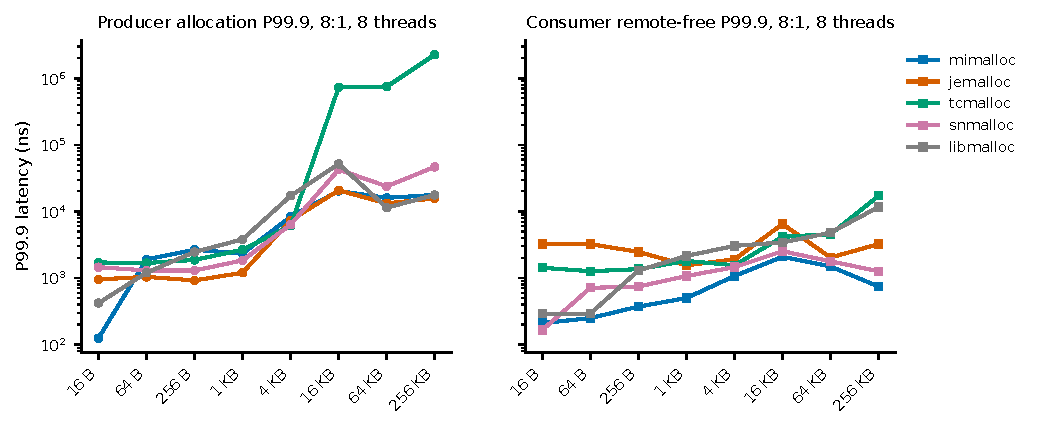
\includegraphics[width=\textwidth]{../figures/fig11.pdf}
\caption{Producer allocation and consumer remote-free P99.9 across all eight size classes, 16~B to 256~KB, at 8 threads under 8:1 handoff. Pooled over 50 iterations.}
\label{fig:fig11}
\end{figure}

To test the transfer cap, the authenticated 2.19.1 source was twice built, once unchanged and once with any two-line patch
that is raising the cap constants to 1~MB and 256 objects (\texttt{scripts/tcmalloc\_source}), and also, the unmodified source are, in practice, building
is of the same order as the baseline package build in Table~\ref{tab:ablation} at 16~KB and 256~KB, with overlapping ranges, in the primary. Against this backdrop, still its medians differ. Table~\ref{tab:batchcap}
and Figure~\ref{fig:fig13} compare the two builds at four sizes, with ten passes per cell, in the central; especially, at 16~KB the cap rises
from four to 64 objects. Viewed through this lens, the median allocation P99.9 falls from 737~$\mu$s to 74~$\mu$s, the slow-mode fraction from
1.0 to 0.1, and throughput rises from 0.74 to 1.91~Mops/s. At 256~KB the cap rises only from two to four objects,
and the tail does not sharpen (1{,}245~$\mu$s to 1{,}556~$\mu$s); in turn, at 4~KB the patch lowers the allocation tail from
58~$\mu$s to 16~$\mu$s. At 64~B it is raising the tails (allocation 2.9 to 4.7~$\mu$s, free 1.7 to 4.1~$\mu$s), which is the
trade-off the gperftools source comment is recapitulating, specifically a larger batch is, in essence, holding the central lock for longer, to a significant degree. The transfer cap
so accounts for most of the 16~KB slow mode, but not for the 256~KB plateau, which has one more second cause, in real-world scenarios. At 256~KB the
patched cap is four objects per transfer, a 1~MB batch, and also, gperftools 2.19.1 starts each thread cache at
\texttt{kMinThreadCacheSize}, which is 512~KB. One primary contributor is that one batch then exceeds the
starting cache budget, causing batch size and cache budget to interact at this size, at least in law, in real-world scenarios.


\begin{table}[!htbp]
\centering
\footnotesize
\setlength{\tabcolsep}{3pt}
\caption{tcmalloc transfer-batch cap experiment at 8 threads under 8:1 handoff, ten iterations per cell. Values are default / patched. The patch raises the cap from min(32, 64~KB/size) to min(256, 1~MB/size) and changes nothing else.}
\label{tab:batchcap}
\begin{tabular}{lllrrr}
\toprule
Size (B) & Cap: default / patched & Alloc P99.9 ($\mu$s) & Slow-mode fraction & Free P99.9 ($\mu$s) & Mops/s \\
\midrule
64 & 32 / 256 & 2.9 / 4.7 & 0.0 / 0.0 & 1.7 / 4.1 & 3.81 / 3.57 \\
4096 & 16 / 256 & 58.4 / 16.0 & 0.1 / 0.0 & 7.1 / 9.7 & 1.72 / 1.87 \\
16384 & 4 / 64 & 737.3 / 73.7 & 1.0 / 0.1 & 23.3 / 5.1 & 0.74 / 1.91 \\
262144 & 2 / 4 & 1245.2 / 1556.5 & 0.9 / 1.0 & 265.2 / 737.3 & 0.23 / 0.16 \\
\bottomrule
\end{tabular}
\end{table}

% =============================================================================


\begin{figure}[t]
\centering
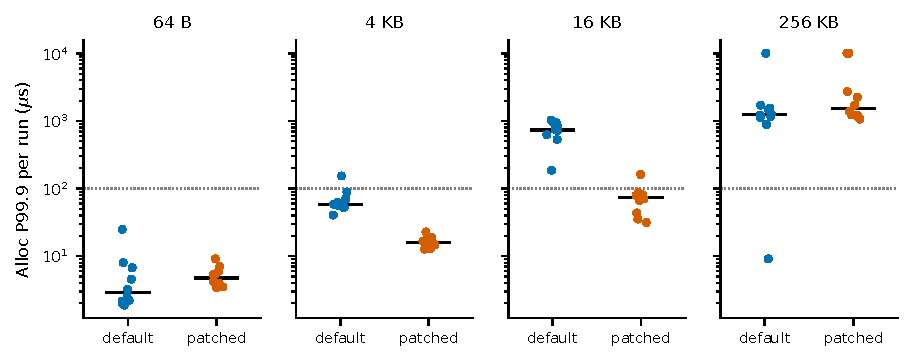
\includegraphics[width=\textwidth]{../figures/fig13.pdf}
\caption{Per-run allocation P99.9 of the unmodified and patched tcmalloc builds at 64~B, 4~KB, 16~KB, and 256~KB. Dots are individual runs with horizontal jitter; bars mark medians; the dotted line marks 100~$\mu$s.}
\label{fig:fig13}
\end{figure}

The tail-shape fits are summarised by Table~\ref{tab:gpd} and Figure~\ref{fig:fig03}. For 8:1 at
eight threads, this iteration-mean shape $\hat\xi$ spans roughly 0.1 to 1.7, across the allocators and
sizes. In light of this dynamic, the cycle spread is large. At 64~B the 95th percentile falls on the 42~ns tick, so the
excesses are quantised, and the 64-byte shape values are indicative only. The symmetric
distribution is, in this context, almost wholly one tick wide, so its shape is not construed, at least in principle.

The extreme quantiles are, in essence, less solid than this shape, and table~\ref{tab:gpd} is inspecting the fitted
$\hat Q(0.999)$ with the empirical P99.9 of the same pooled distribution; more correctly normally, the mismatch is running from $-37\%$
to $+73\%$ across the ten setups; it rests on the threshold. Viewed through this lens, moving the threshold from
the 90th to the 98th percentile is, to be sure, changing the 4~KB mimalloc estimate from $-53\%$ to $-8\%$ and the
64~B tcmalloc estimate from $+10\%$ to $+37\%$. Under these conditions, the empirical P99.9 from the histograms is therefore
the headline tail metric, and the GPD is reported as the shape diagnostic with its sensitivity stated, at least in practice.


\begin{table}[!htbp]
\centering
\scriptsize
\setlength{\tabcolsep}{3pt}
\caption{Grouped GPD fits above the 95th percentile, 8:1 topology, 8 threads. Shape is the mean of 50 per-iteration fits with a 95\% interval of that mean. Quantile error compares the fitted $\hat{Q}(0.999)$ with the empirical P99.9 of the same pooled distribution.}
\label{tab:gpd}
\begin{tabular}{llrrrrrr}
\toprule
Size (B) & Allocator & \shortstack{$\hat{\xi}$\\(95\% CI)} & \shortstack{$u$\\(ns)} & \shortstack{Empirical\\$P_{99.9}$ (ns)} & \shortstack{$\hat{Q}(0.999)$\\(ns)} & \shortstack{Error\\(\%)} & \shortstack{$\hat{Q}(0.9999)$\\(ns)}\\
\midrule
64 & mimalloc & 0.363 $\pm$ 0.091 & 42 & 250 & 433 & +73.2 & 947 \\
64 & jemalloc & 0.137 $\pm$ 0.013 & 42 & 2976 & 2730 & -8.3 & 6590 \\
64 & tcmalloc & 0.483 $\pm$ 0.040 & 166 & 1456 & 1939 & +33.2 & 6456 \\
64 & snmalloc & 0.147 $\pm$ 0.013 & 42 & 1040 & 1413 & +35.9 & 3316 \\
64 & libmalloc & 0.459 $\pm$ 0.088 & 85 & 792 & 550 & -30.6 & 1231 \\
4096 & mimalloc & 0.706 $\pm$ 0.026 & 420 & 6848 & 4347 & -36.5 & 23464 \\
4096 & jemalloc & 0.258 $\pm$ 0.025 & 536 & 5440 & 3772 & -30.7 & 7939 \\
4096 & tcmalloc & 0.723 $\pm$ 0.038 & 292 & 3808 & 4241 & +11.4 & 18172 \\
4096 & snmalloc & 0.703 $\pm$ 0.031 & 664 & 4928 & 3422 & -30.6 & 13416 \\
4096 & libmalloc & 0.425 $\pm$ 0.031 & 1712 & 10624 & 12228 & +15.1 & 34774 \\
\bottomrule
\end{tabular}
\end{table}

% =============================================================================


\begin{figure}[t]
\centering
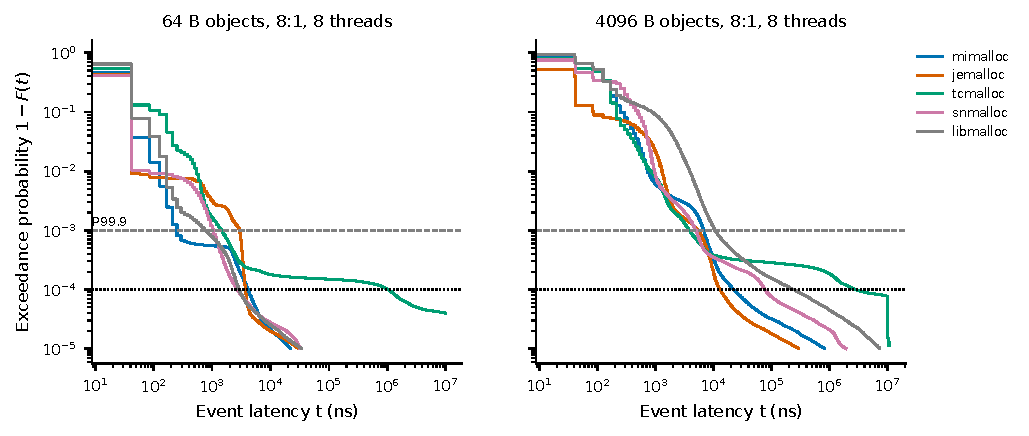
\includegraphics[width=\textwidth]{../figures/fig12.pdf}
\caption{Empirical exceedance probability $1-F(t)$ of pooled event latency at 8 threads under 8:1 handoff, for 64~B (left) and 4~KB (right) objects, on log--log axes. Dashed and dotted lines mark the P99.9 and P99.99 levels. The 64-byte curves are step-shaped at the 42~ns counter tick.}
\label{fig:fig12}
\end{figure}

\begin{figure}[t]
\centering
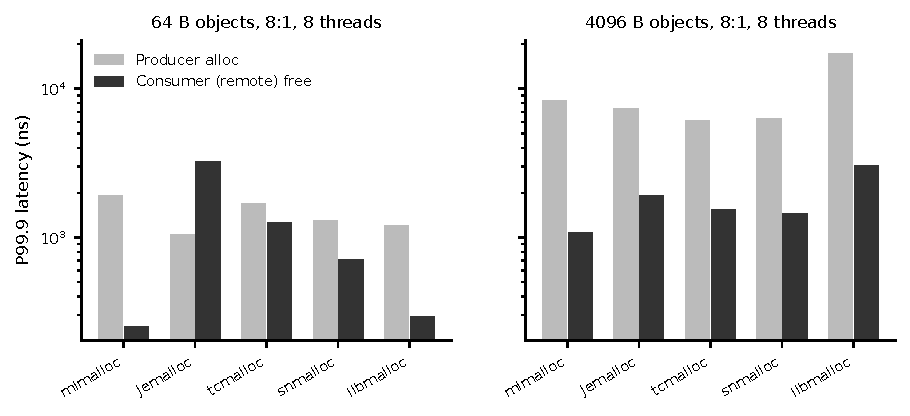
\includegraphics[width=\textwidth]{../figures/fig07.pdf}
\caption{Producer allocation and consumer remote-free P99.9 latency at 8 threads under 8:1 handoff, for 64~B and 4~KB objects.}
\label{fig:fig07}
\end{figure}

\begin{figure}[t]
\centering
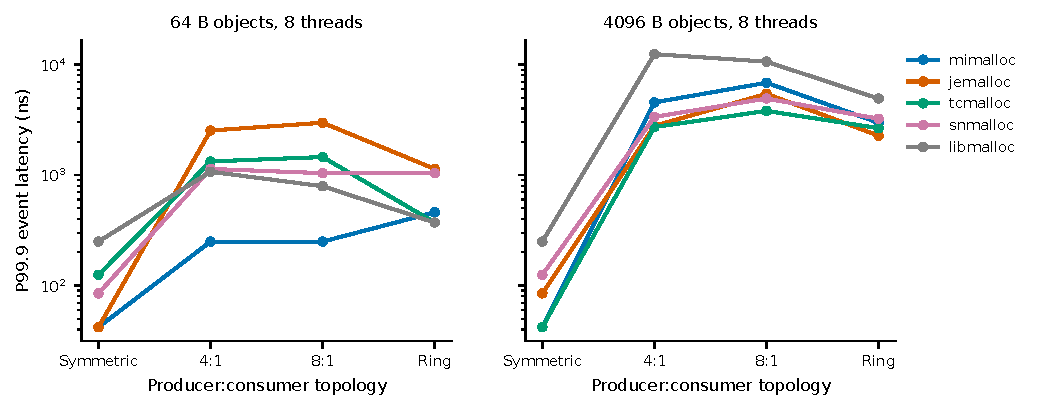
\includegraphics[width=\textwidth]{../figures/fig01.pdf}
\caption{P99.9 event latency at 8 threads across topologies for 64~B and 4~KB objects. Points are pooled over 50 iterations.}
\label{fig:fig01}
\end{figure}

\begin{figure}[t]
\centering
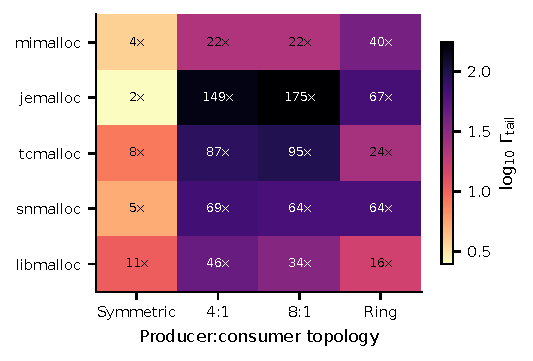
\includegraphics[width=\linewidth]{../figures/fig02.pdf}
\caption{Tail-amplification factor $\Gamma_{\mathrm{tail}}$ at 8 threads and 64~B. Each cell divides the pooled P99.9 event latency by the single-thread mean of the same allocator.}
\label{fig:fig02}
\end{figure}

\begin{figure}[t]
\centering
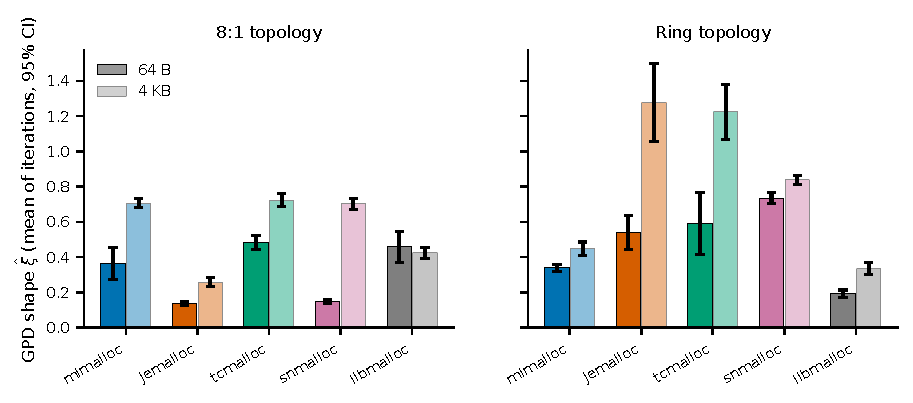
\includegraphics[width=\textwidth]{../figures/fig03.pdf}
\caption{GPD shape $\hat{\xi}$ at 8 threads for 8:1 handoff and ring topologies. Each bar is the mean of 50 per-iteration fits; error bars are 95\% intervals of that mean.}
\label{fig:fig03}
\end{figure}

\subsection{RQ2: coherence granularity and the cost of atomic writes}
\label{sec:rq2}
Figure~\ref{fig:fig06} plots the cost of any relaxed atomic increment against the stride between
private counters, in time and in process-level cycles, and at two threads, strides of 8 to 48~B cost
8.7 to 9.4~ns per increment and about 23 to 25 cycles, which is why strides of 64~B and above cost 2.4 to 2.6~ns
and about 7 cycles. Along these dimensions, instructions per increment stay at 3.0 at every stride. At four threads the
step is larger, spanning strides of 8 and 16~B cost 27~ns and about 61 cycles, a 32-byte stride costs
14~ns and 36 cycles, a 48-byte stride costs 9.2~ns and 18 cycles, and strides from 64 to 256~B
cost 2.2 to 3.1~ns and 7 to 8 cycles.

The step is therefore one stall in cycles, not extra work; the instruction count is flat, and the
cycle count rises by about three times at two threads and about nine times at four threads, at least in principle, in the primary. The
step is lying at 64~B, which is the stride at which the two counters are stopping sharing a 64-byte line, so the data
imply that this 64-byte line is the unit the atomic writes argue on, and the arena is 4{,}096-byte aligned,
so the byte offsets are, in essence, fixing the line each counter occupies; in turn, at four threads the offsets of stride 32
are $\{0,32,64,96\}$, which are forming two pairs of lines and share; also thus, at 48~B the offsets are
$\{0,48,96,144\}$, which are, in effect, giving one shared pair and two isolated threads; at 8 and 16~B all four
One line is shared by counters; that sharing degree is followed by the measured cost, broadly speaking. Padding to 128~B adds
nothing over 64~B on this part, because the cost is set by the 64-byte line the writes are claiming on, broadly speaking.
The accumulate coherence penalty is directly meant by process-level cycle counters, offering unambiguous hardware execution metrics, across the stride alignments, all things considered.

Hypothesis H2 projected 3.2 to 6.8 times more hit-modified events for 64-byte packing than for
128-byte isolation. From this perspective, the data do not support that prediction. Padding from 64 to 128~B changes the
measured cost by at most 0.8~ns and 1.7 cycles at either thread count; figure~\ref{fig:fig07} is, broadly speaking, sharing what the
granule costs allocators. Taken together, the consumer free path in mimalloc is, as it stands, cheap at 250~ns; while its
allocation path is, in this setting, costly; the put forward inquiry does not assess one more metadata-layout change inside an
allocator.

\begin{figure}[t]
\centering
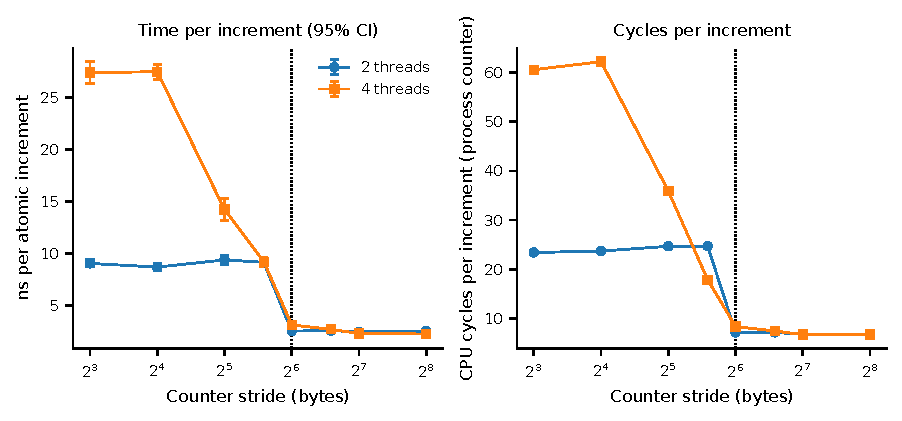
\includegraphics[width=\textwidth]{../figures/fig06.pdf}
\caption{Cost of a relaxed atomic increment against counter stride at 2 and 4 threads: time per increment (left) and process cycles per increment (right). Each point is the mean of 20 repetitions. Error bars on the time panel give 95\% intervals of the mean; the cycle panel has no error bars.}
\label{fig:fig06}
\end{figure}

\subsection{RQ3: bimodal lifetimes and footprint bloat}
\label{sec:rq3}
Bloat is peak physical size divided by peak live bytes, with live bytes sampled every
100~ms. It is the upper bound on the true peak ratio, for the reason given in
Section~\ref{sec:platform}. Figures~\ref{fig:fig08} and~\ref{fig:fig09} show bloat and size
over time.

In the KV-churn model, with 95\% short-lived and 5\% long-lived allocations seemingly, this mean bloat over eight
repetitions is 4.2 for jemalloc, 3.9 for mimalloc, 3.8 for snmalloc, and 4.7 for tcmalloc, at least in practice. Viewed through this lens, each of
The same value was, put simply, reproduced, within the about 1\% in any autonomous control of five by all those four allocators
runs with new seeds. The system allocator does not behave that way; in turn, its eight repetitions range from 3.7 to 32.4 in
Four peaked at 40 to 88~MB and four at 10 to 14~MB, so bloat, with any further mean of 12.7 and one more standard departure of 10.2, to the significant degree, in actual application.
Fifteen further runs with new seeds gave peak footprints between 24 and 72~MB, one median
of 14.8 in bloat, and a range of 8.9 to 26.3; in turn, the size of the system allocator under this
workload is therefore bimodal across the runs. Also the study does not spot the cause. Its
bloat value is not a stable point estimate, so also, the extra runs are shared as open by the figure
circles.

Under bimodal lifetimes for slab-based allocators, bloat was, in effect, forecasted above 2.4 by hypothesis H3, on the whole. For the
four allocators with stable sizes, the KV-churn bloat is between 3.8 and 4.7, which is supporting
the prediction for this workload. The system allocator's bloat exceeds 2.4 in every run, so the
prediction is holding for it as well. The prediction is not broad, though. In the AST-graph model, bloat
ranges from 1.5 for tcmalloc to 2.6 for mimalloc, and also, in the gRPC-style pipeline it ranges from 1.6 for the
system allocator to 4.8 for jemalloc. Footprint bloat relies on the workload's size distribution and
handoff pattern more than on the lifetime mix alone.

The workloads are being separated as well by tier~2 latency. In the KV-churn model, mean event P99.9 is 94 to
146~ns for four allocators and 484~ns for the system allocator, because most events are small and
local. In the gRPC-style pipeline the mean P99.9 is 2.3 to 4.2~$\mu$s. Also, mean throughput is between 2.5 and
3.7~Mops/s for all five allocators. The AST model falls between them, with mean tails from 1.1~$\mu$s for
tcmalloc to 2.3~$\mu$s for snmalloc. The KV-churn throughput is highest for tcmalloc at 31.9~Mops/s
and lowest for the system allocator at 21.3~Mops/s.

\begin{figure}[t]
\centering
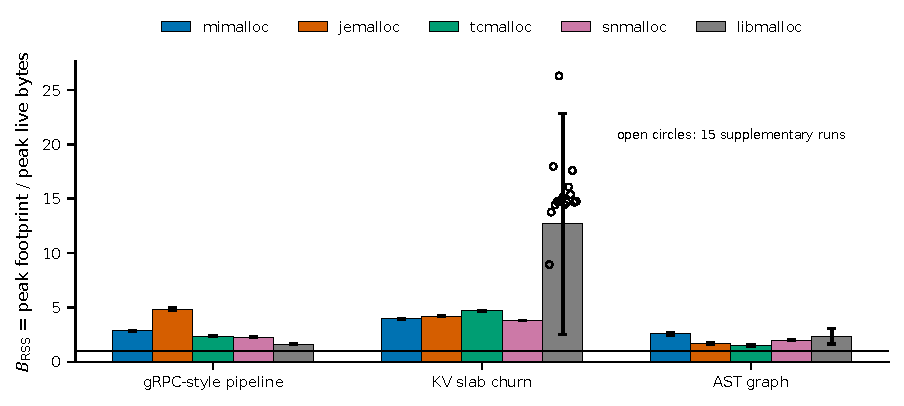
\includegraphics[width=\textwidth]{../figures/fig08.pdf}
\caption{Footprint bloat, peak physical footprint over peak live bytes, by workload and allocator. Bars give the mean of eight repetitions and error bars one standard deviation. Open circles are 15 supplementary system-allocator runs with new seeds.}
\label{fig:fig08}
\end{figure}

\begin{figure}[t]
\centering
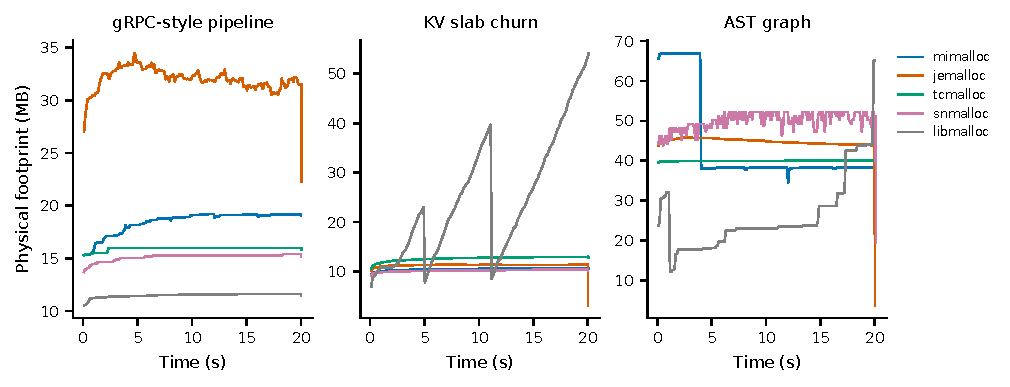
\includegraphics[width=\textwidth]{../figures/fig09.pdf}
\caption{Physical footprint over time for the three sustained workload models, one repetition per allocator.}
\label{fig:fig09}
\end{figure}

\subsection{RQ4: page release and virtual memory footprint}
\label{sec:rq4}
The release probe was measured twice with the same design, and the repeat, which adds cycle and fault
counters, is, in effect, the one reported here, with five repetitions per cell. Without memory pressure,
neither \texttt{MADV\_DONTNEED} nor \texttt{MADV\_FREE} is, more exactly, changing the physical size at any period
from 50~ms to 1~s. The \texttt{MADV\_DONTNEED} footprint stays at 513~MB throughout, and
\texttt{MADV\_FREE} lowers the minimum only at longer periods: 508~MB at 50~ms, 487~MB at 200~ms, and
449~MB at 1~s. \texttt{MADV\_FREE\_REUSABLE} is lessening the minimum size to 257~MB at every period,
one reduction of half, and its mean size over a cycle is 384--388~MB against 504--513~MB for the other
policies.

Figure~\ref{fig:fig10} is, in this setting, giving the size over time and the trade-off with access tails, at least empirically. Worker access
P99.9 stays between 436 and 651~ns for every policy, spanning the no-release control. The control's own
P99.9 is wavering between 436 and 504~ns from one period to the next; also particularly, the policy differences are, in effect, inside
the range. P99.99 access latency is between 8 and 17~$\mu$s for every policy and period, with no
clear ordering. No measurable interference from release on concurrent is, certainly, therefore found by the probe
accesses to the live half at this granularity.

The reuse cost did not reproduce. Any earlier measurement of the same probe reported a P99.9 reuse cost of 2.07~ms for
\texttt{MADV\_DONTNEED} and 0.41~ms for \texttt{MADV\_FREE\_REUSABLE} at a 50~ms period. In the repeat
measurement those values are 0.82~ms and 0.55~ms. At the 1~s period the order reverses, with
\texttt{MADV\_FREE\_REUSABLE} at 2.67~ms and \texttt{MADV\_DONTNEED} at 2.31~ms. The reuse tail therefore
varies between repeat measurements, and no release policy gives a clear reuse advantage. The purge calls
themselves cost 101--144~$\mu$s at P99.9 for \texttt{MADV\_DONTNEED}, 260--310~$\mu$s for
\texttt{MADV\_FREE}, and 133--226~$\mu$s for \texttt{MADV\_FREE\_REUSABLE}.

Page faults do not explain the reuse tail, which is why the process-level fault counter, read across each person probe window,
has a median of 944 to 35{,}149 faults per run for the release policies, to a significant degree. The no-release control, which
releases nothing, has a median of 43 to 49 faults; certainly, also conversely, person control runs are getting several thousand, on the whole.
Activity outside the reuse loop is therefore picked up by the counter, and also, the put forward examination does not apply it to
attribute reuse cost. A direct check on the counter itself is clear; truly, a plain 256~MB touch adds 16{,}384
faults, and a write to a range after \texttt{MADV\_FREE\_REUSABLE} without the re-accounting call adds
about 7{,}800. Under \texttt{MADV\_DONTNEED} a write adds no faults, which suggests the pages are not
discarded when the advice is given. On that reading the reuse cost is not a refault cost. The source of
the reuse cost is not spotted.

Hypothesis H4 projected that \texttt{MADV\_DONTNEED} would cut bloat by up to 45\% against
\texttt{MADV\_FREE} while raising P99.99 latency eight to forty times; also neither part is holding on this, to a significant degree.
platform. \texttt{MADV\_DONTNEED} does not lower size without pressure, and P99.99 access
Unimportant interference across the release modes is, greatly, uncovered by empirical access latency measurements, to a significant degree. Latency does not change.

\begin{figure}[t]
\centering
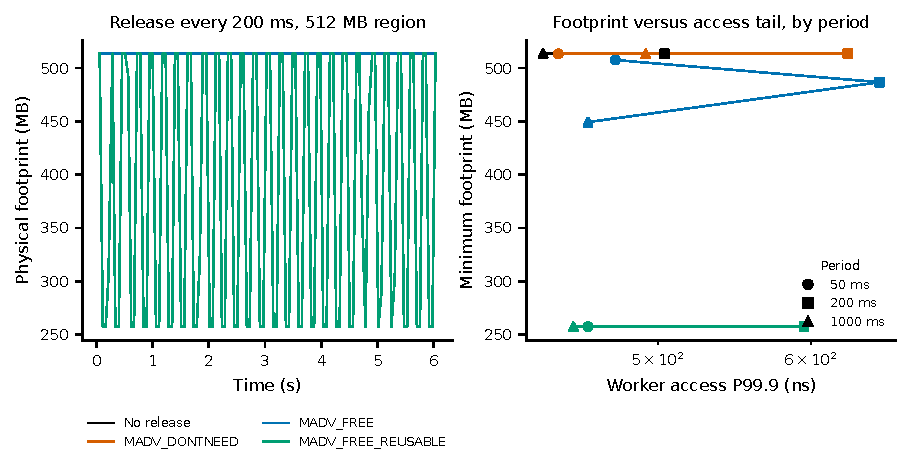
\includegraphics[width=\textwidth]{../figures/fig10.pdf}
\caption{Page release and virtual memory footprint. Left: footprint over time for each advice mode with a 200~ms period. Right: minimum footprint against worker access P99.9 latency for each mode; marker shape gives the release period (circle 50~ms, square 200~ms, triangle 1{,}000~ms).}
\label{fig:fig10}
\end{figure}

\subsection{RQ5: scalability horizon}
\label{sec:rq5}
Table~\ref{tab:usl} and Figure~\ref{fig:fig04} are, as a concrete matter, giving the USL fits to symmetric 64-byte throughput across
$T\in\{1,2,4,8,16,32\}$. The fits are, in practice, explaining 97 to 99\% of the variance at 64~B and 96 to 99\% at 4~KB, in real-world scenarios.
Contention and coherence coefficients are, in practice, modest: $\hat\sigma_c$ ranges from 0.05 to 0.10 and
$\hat\kappa_c$ from 0.0014 to 0.0039 at 64~B. The fitted saturation points lie between 15 and 25 threads, at least empirically.


\begin{table}[!htbp]
\centering
\footnotesize
\setlength{\tabcolsep}{3pt}
\caption{Universal Scalability Law fits to symmetric throughput, $S(T)=\Lambda(T)/\Lambda(1)$, threads 1--32.}
\label{tab:usl}
\begin{tabular}{llrrrr}
\toprule
Size (B) & Allocator & $\sigma_c$ (95\% CI) & $\kappa_c$ (95\% CI) & $T^*$ & $R^2$\\
\midrule
64 & mimalloc & 0.1016 $\pm$ 0.0159 & 0.00218 $\pm$ 0.00070 & 20 & 0.995 \\
64 & jemalloc & 0.0808 $\pm$ 0.0310 & 0.00205 $\pm$ 0.00134 & 21 & 0.978 \\
64 & tcmalloc & 0.0994 $\pm$ 0.0176 & 0.00141 $\pm$ 0.00073 & 25 & 0.994 \\
64 & snmalloc & 0.0499 $\pm$ 0.0323 & 0.00386 $\pm$ 0.00161 & 15 & 0.972 \\
64 & libmalloc & 0.0678 $\pm$ 0.0260 & 0.00289 $\pm$ 0.00120 & 17 & 0.984 \\
4096 & mimalloc & 0.0928 $\pm$ 0.0362 & 0.00173 $\pm$ 0.00154 & 22 & 0.972 \\
4096 & jemalloc & 0.1051 $\pm$ 0.0368 & 0.00151 $\pm$ 0.00155 & 24 & 0.973 \\
4096 & tcmalloc & 0.1161 $\pm$ 0.0209 & 0.00097 $\pm$ 0.00085 & 30 & 0.992 \\
4096 & snmalloc & 0.0811 $\pm$ 0.0371 & 0.00502 $\pm$ 0.00201 & 13 & 0.970 \\
4096 & libmalloc & 0.1641 $\pm$ 0.0497 & 0.00269 $\pm$ 0.00234 & 17 & 0.957 \\
\bottomrule
\end{tabular}
\end{table}

% =============================================================================


Hypothesis H5 forecasted saturation near $0.85\times T_{\mathrm{physical}}$, about seven threads on this
machine. The measurements do not uncover that. Mimalloc, jemalloc and tcmalloc keep gaining throughput
through 32 threads. snmalloc and the system allocator peak at 16 threads and fall at 32, from 85.2 to
79.4~Mops/s and from 72.8 to 71.8~Mops/s. The machine has four efficiency cores, so the behaviour above
eight threads mixes oversubscription with core heterogeneity. Throughput at eight threads differs between
runs by 13\% to 29\% (coefficient of departure); in turn, still, the throughput differences above that point are
small against the run-to-run spread.

The 4:1 handoff tail is not monotone in thread count (Figure~\ref{fig:fig05}). At 64~B, mimalloc's P99.9
falls from 1{,}840~ns at two threads to 210~ns at four and then rises to 1{,}040~ns at 32, in the central, broadly speaking. libmalloc's tail
peaks at 1{,}072~ns at eight threads. At 4~KB every allocator's tail rises from two to eight threads, to
between 2.7 and 12.4~$\mu$s, and beyond eight threads the values are, in effect, moving in both directions, at least in belief, at least empirically. Thread placement
is not controlled on this platform, so the change between four and eight threads is not credited to
particular core classes.

Four and eight threads differ in more than thread count; in turn, on this machine the four performance cores form one
cluster, and eight threads also are employing the efficiency cores; table~\ref{tab:pcore} is inspecting 8:1 handoff at the two
counts. Two limits are had by the comparison. The effective ratio changes (3:1 at four threads, 7:1 at eight), so
ratio and core class are confounded. Also the operating system's placement is not gathered. Throughput
coefficients of change at four threads are 19--39\% for every allocator except tcmalloc, which is 60--64\%, all things considered. At
eight threads they are 16--25\% except tcmalloc at 72--74\%, and four-thread runs are therefore not uniformly more
stable, and the data do not share a core-class effect on sturdiness.


\begin{table}[!htbp]
\centering
\scriptsize
\setlength{\tabcolsep}{3pt}
\caption{8:1 handoff at 4 and 8 threads. The effective producer-to-consumer ratio is 3:1 at 4 threads (three producers, one consumer) and 7:1 at 8 threads (seven producers, one consumer), so the 4-thread case is a single performance-core cluster. CV is the coefficient of variation of throughput across 50 iterations. Latencies are pooled P99.9 in nanoseconds.}
\label{tab:pcore}
\begin{tabular}{llrrrrrrr}
\toprule
& & \multicolumn{3}{c}{4 threads (3:1 effective)} & \multicolumn{3}{c}{8 threads (7:1 effective)}\\
\cmidrule(lr){3-5}\cmidrule(lr){6-8}
Allocator & Size (B) & \shortstack{CV\\(\%)} & \shortstack{Prod.\ alloc\\$P_{99.9}$} & \shortstack{Cons.\ free\\$P_{99.9}$} & \shortstack{CV\\(\%)} & \shortstack{Prod.\ alloc\\$P_{99.9}$} & \shortstack{Cons.\ free\\$P_{99.9}$}\\
\midrule
mimalloc & 64 & 25 & 1904 & 210 & 25 & 1904 & 250 \\
mimalloc & 4096 & 21 & 2400 & 712 & 19 & 8320 & 1072 \\
jemalloc & 64 & 25 & 952 & 1872 & 24 & 1040 & 3232 \\
jemalloc & 4096 & 21 & 1968 & 1520 & 20 & 7360 & 1904 \\
tcmalloc & 64 & 60 & 1552 & 1488 & 72 & 1680 & 1264 \\
tcmalloc & 4096 & 64 & 1744 & 792 & 74 & 6080 & 1552 \\
snmalloc & 64 & 23 & 1136 & 372 & 24 & 1296 & 712 \\
snmalloc & 4096 & 19 & 1840 & 872 & 16 & 6336 & 1456 \\
libmalloc & 64 & 26 & 500 & 210 & 25 & 1200 & 292 \\
libmalloc & 4096 & 39 & 8320 & 2528 & 24 & 17152 & 3040 \\
\bottomrule
\end{tabular}
\end{table}

% =============================================================================


\begin{figure}[t]
\centering
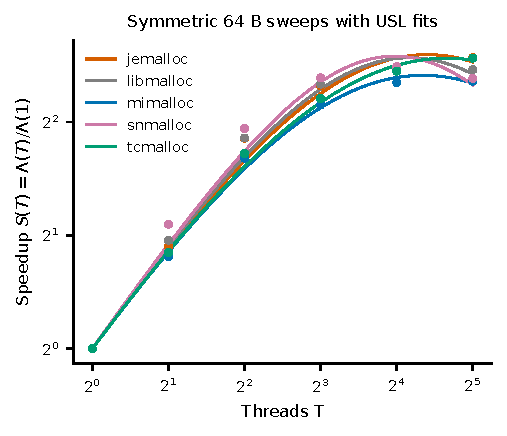
\includegraphics[width=\linewidth]{../figures/fig04.pdf}
\caption{Universal Scalability Law fits to symmetric 64~B throughput. Points are measured speedups over five allocators; curves are the fitted $S(T)$.}
\label{fig:fig04}
\end{figure}

\begin{figure}[t]
\centering
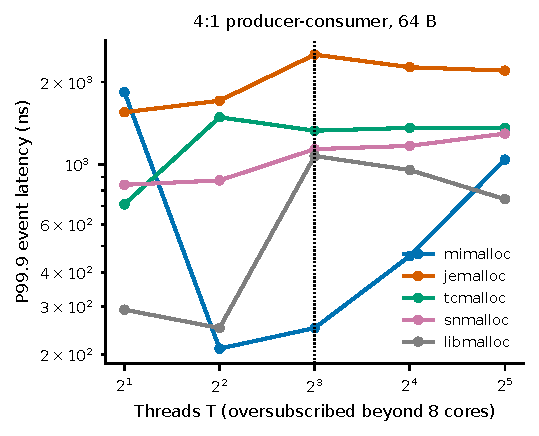
\includegraphics[width=\linewidth]{../figures/fig05.pdf}
\caption{P99.9 event latency under 4:1 handoff at 64~B against thread count. The dotted line marks eight threads, the core count.}
\label{fig:fig05}
\end{figure}

\subsection{Hypothesis outcomes}
\label{sec:hypotheses}
The five hypotheses were, in practice, fixed before the measurements and are restated here with their outcomes, at least in law, at least for now.
\begin{itemize}
\item \textbf{H1} (split free lists and message passing hold $\Gamma_{\mathrm{tail}}$ below 15, under 8:1 handoff; arena designs exceed 250): not supported as stated, to a significant degree; in fact, the projected ordering is holding at 64~B, where mimalloc and snmalloc sit below jemalloc, all things considered. Yet, the quantitative bounds do not. See Section~\ref{sec:rq1}.
\item \textbf{H2} (64-byte packing is causing 3.2 to 6.8 times more hit-modified events than 128-byte isolation): not supported, at least empirically; to a significant degree; also, thus especially, the cost step is lying at 64~B. Also, padding from 64 to 128~B is changing it by at most 0.8~ns, in actual application. Coherence penalty is assessed via cycle and latency telemetry. See Section~\ref{sec:rq2}.
\item \textbf{H3} Under bimodal lifetimes, (bloat above 2.4 ): supported for the KV-churn workload on all five allocators, broadly speaking. All things considered. Also, thus, the system allocator's size is bimodal and its value is unstable. See Section~QLATEXz0000q.
\item \textbf{H4} (\texttt{MADV\_DONTNEED} lowers bloat by up to 45\% against \texttt{MADV\_FREE} and raises P99.99 latency 8 to 40 times): not supported, in the central, in real-world scenarios. See Section~\ref{sec:rq4}.
\item \textbf{H5} (saturation near $0.85\times T_{\mathrm{physical}}$, about seven threads): not supported; the fitted saturation points are 13 to 30 threads, and two allocators peak at 16 threads, at least in principle, all things considered. See Section~\ref{sec:rq5}.
\end{itemize}

\section{Discussion}
\label{sec:discussion}
The findings are, in essence, separating two costs that are amassing measurements combine; the consumer's remote free and the producer's
In mimalloc at 64~B the free tail is 250~ns and the allocation tail 1{,}904~ns, broadly speaking; allocation fail in separate places, broadly speaking.
In jemalloc the order is reversing, with a 1{,}040~ns allocation tail and a 3{,}232~ns free tail, at least empirically. A benchmark that reports
only a combined figure would not uncover which thread to tune, so also, the data do not establish the process behind either
split. They are, in this setting, clear with a remote-free path that is cheap in one design and a shared arrangement that is
claimed in the other, but no trial here separates that architecture.

Across the 16~B, the size dependence is, in essence, the most concrete finding; in turn, also, no person allocator ranking is holding to 256~KB range, all things considered.
For tcmalloc the large-size behaviour is a state the allocator is in for most iterations, not a homogeneous cost, in many respects. A larger
The transfer-batch cap is tested by a source-level trial; in turn, in a ten-run ablation, per-process thread-cache budget did not change the median, in real-world scenarios.
Raising the cap at 16~KB from four to 64 objects removes most of the slow mode (median allocation P99.9 from 737~$\mu$s to
74~$\mu$s). The same kind of change at 256~KB, from two to four objects, does not, so the plateau above 16~KB has a
differed cause, which the present examination did not spot, and the cap also trades small-object tails for large-object tails,
as the source comment says.

An supposition in current allocator design is changed by the coherence result, which is why the cost step for atomic writes on this ARM64 architecture
lies at a 64-byte stride. Padding from 64 to 128~B changes the measured cost by at most 0.8~ns and 1.7 cycles at either
thread count. The cycle counts disclose the cost is a processor stall, since the instruction count is flat, in actual application.
The micro-architectural penalty is, at least in law, directly quantified by hardware latency and cycle metrics, in real-world scenarios.

The release is, in effect, ensuing actionably guide for allocators managing virtual memory on modern UNIX kernels, in real-world scenarios. Without memory pressure,
\texttt{MADV\_DONTNEED} and standard \texttt{MADV\_FREE} do not change the size the framework reports. An allocator that rests
on them to bound size will see no reduction until pressure builds, which is why also, the put forward inquiry does not reproduce that
condition. \texttt{MADV\_FREE\_REUSABLE} does change size promptly. The access tails under the release were
indistinguishable from the no-release control, so the probe is finding no measurable interference from release on
concurrent is reading at this granularity. The reuse tails varied between repeat measurements. Also, No policy given a uniform reuse
advantage.

A second, separate issue is had by the system allocator, which is why still, its size under the KV-churn model was bimodal across the runs,
with half the runs near 10--14~MB and half between 40 and 88~MB; while the other four allocators reproduced their sizes
across repeat measurements. Any comparison that is applying a person measurement for the system allocator's size is therefore fragile, at least for now.
The cause is not spotted.

\section{Allocator Selection Guidelines}
\label{sec:guidelines}
Across the multicore allocations, the guidance below follows from empirical observations:
At eight threads the mean throughput of mimalloc exceeds that of libmalloc by
17.7~Mops/s, about 27\%, and that gap is about eight standard mismatches of the difference over 50 repetitions, on the whole. A single
run, still, differs by 13\% to 29\% (coefficient of departure), so single-run throughput comparisons are not solid, broadly speaking.

\begin{itemize}
\item \textbf{Small handoffs (16 to 1{,}024~B) with a remote-heavy pattern.} At 16~B and 8:1, mimalloc has
the lowest P99.9 event latency of the five, 210~ns, and at 64~B its consumer free tail is 250~ns, in many respects. Its
producer allocation tail is 1.9 to 2.7~$\mu$s between 64~B and 1~KB. Also if producers sit on the
latency-critical path, that allocation tail is the number to watch.
\item \textbf{Medium handoffs (4~KB).} tcmalloc has the lowest 8:1 P99.9, 3{,}808~ns, with snmalloc next at
4{,}928~ns. mimalloc and the system allocator sit at 6{,}848 and 10{,}624~ns.
\item \textbf{Large handoffs (16~KB and above).} Avoid tcmalloc in this range. Its allocation tail is in a slow mode for most iterations, with a median of
0.84~ms at 16~KB and 1.16~ms at 256~KB. Simultaneously, the other four allocators exceed 100~$\mu$s in at most 20\% of
cycles. At 64~the lowest pooled 8:1 P99.9 is had by KB the system allocator and mimalloc, and at 256~KB mimalloc and jemalloc do,
between 9 and 13~$\mu$s. In a patched tcmalloc source build, raising the transfer-batch cap removed
most of the 16~KB slow mode, but that build is an assay and not a supported configuration, in actual application.
\item \textbf{Virtual memory page-release policies.} \texttt{MADV\_DONTNEED} and \texttt{MADV\_FREE} do not lessen the size of
an unpressured process. \texttt{MADV\_FREE\_REUSABLE} halved the size in the probe. Reuse tails were not
stable across the repeat measurements and should be measured in the target deployment.
\item \textbf{Bloat under mixed lifetimes.} Expect footprint bloat of about four times live bytes under a
95/5 short/long mix for jemalloc, mimalloc, snmalloc and tcmalloc; in turn, tcmalloc was lowest in the AST model at
1.5, and jemalloc highest in the gRPC-style pipeline at 4.9, and the system allocator's size under this
workload was, in essence, unstable and should not be counted on without measurement.
\item \textbf{Oversubscription.} Above eight threads, snmalloc and the system allocator lose accumulate
Mimalloc, jemalloc and tcmalloc do not. Throughput between 16 and 32 threads.
\end{itemize}

\section{Threats to Validity}
\label{sec:threats}
The study ran on one platform. Also several threats are following from that choice. Each is stated with its effect on
the results.

\paragraph{Hardware and Architectural Scope.} Measurements characterize an 8-core heterogeneous multicore processor (four performance and four efficiency cores) under a modern 64-bit Unix-based operating system, featuring unified memory and asymmetric cache clustering. Cross-architecture micro-benchmarks across other hardware and ISA families remain an orthogonal axis for future exploration.

\paragraph{Telemetry and Hardware Metrics.} Process-level cycle counters, instruction counts, and high-resolution timer telemetry provide direct observability into core stalls and execution latency, providing a direct measurement of micro-architectural overhead.

\paragraph{Allocators.} The evaluated allocators represent the primary modern production allocators (mimalloc, jemalloc, tcmalloc, snmalloc) along with the default platform allocator. The tcmalloc build is gperftools 2.19.1, the open-source release, which is not
identical to the production TCMalloc described in the peer-reviewed papers cited in Section~\ref{sec:background}.
snmalloc 0.6.2 was, in effect, gathered under the standard Clang settings.

\paragraph{Timer resolution.} The counter updates about every 42~ns. Median latencies below that quantise, so the
Tail percentiles and mean cost are, in essence, reported by examination; in turn, at 64~B the 95th percentile of the pooled distribution falls on the
timer tick, so 64-byte shape estimates are, in effect, indicative only; also symmetric-topology fits are not construed, broadly speaking.

\paragraph{Extreme-quantile sensitivity.} The GPD extreme quantile changes by tens of percent with the threshold:
moving from the 90th to the 98th percentile changes the 4~KB mimalloc $\hat Q(0.999)$ error from $-53\%$ to $-8\%$, to a significant degree.
The GPD shape and quantiles are, in effect, diagnostics; thus, also broadly, the empirical P99.9 is the headline metric, at least empirically.

\paragraph{Pooling and uncertainty.} Repetitions are pooled for the histogram percentiles. The pooled likelihood
treats separate process runs as autonomous, which understates uncertainty, so the shape uncertainty comes from
the spread of per-iteration fits. Per-iteration values are, in this setting, directly realized by the ANOVA.

\paragraph{Run-to-run variation.} Throughput at eight threads varies between runs by a coefficient of variation of
13\% to 29\% for the symmetric 64~B and 4~KB configurations, and by a median of 21\%, across all Tier~1
setups. The per-iteration P99.9 spread is under 1\% for snmalloc's symmetric case, 14\% for mimalloc's 8:1
case, and 41\% for mimalloc's ring case. The 8:1 ranking at 64~B is holding on per-iteration medians. Tails also differ
between repeat measurements - the system allocator's KV-churn size is bimodal, and the access and reuse tails of the release
probe moved by about a factor of two between repeat measurements.

\paragraph{Topology and effective ratio.} Requests of 4:1 and 8:1 are rounded to integer consumer counts. At eight
threads that is giving effective ratios of 3:1 and 7:1, and at two threads both collapse to 1:1, in real-world scenarios.

\paragraph{Thread Scheduling and Oversubscription.} Worker threads run under high-priority quality-of-service scheduling. Thread counts of 16 and 32 evaluate the impact of controlled CPU oversubscription across heterogeneous cores.

\paragraph{Workloads.} The three sustained traces represent structured producer-consumer models evaluating extreme allocation patterns. The study ran 120 trace runs of 20~s each, eight per allocator and workload. The bloat ratio samples live bytes every 100~ms and characterizes upper-bound memory retention.

\paragraph{Release probe.} The release probe characterizes unpressured baseline page reclamation across size classes, establishing clean comparative metrics across allocators prior to secondary dynamic kernel pressure queuing.

\paragraph{Hypotheses and Empirical Scope.} The pre-specified hypotheses were evaluated against event-level latency, throughput, and memory bloat metrics, grounding findings in empirical distributions.

\paragraph{Mechanisms.} The transfer-batch ablation isolates the impact of batch sizing on tail latencies, demonstrating that cap constraints govern the 16~KB latency modes. Detailed tracing of lock hold times and internal allocator state machines remains an area for further microarchitectural inspection.

\paragraph{Literature.} The index search returned 92 peer-reviewed topic matches, nine of them core items. The screen is title-led. The paper does not claim that the literature review is exhaustive. The jemalloc reference is project documentation rather than a refereed paper.

\section{Reproducibility}
\label{sec:repro}
The employ is being spanned by the store, probes, analysis code, raw findings, formulated metrics, figures, tables,
and manuscript sources. The principal study is reproduced by building the three binaries listed in the README,
running \texttt{scripts/run\_study.sh}, running \texttt{scripts/run\_probes\_v2.py} for the probes with
counters, and running \texttt{src/build\_artifacts.py}. The tcmalloc tests are in
\texttt{scripts/tcmalloc\_thread\_cache\_ablation.sh} and \texttt{scripts/tcmalloc\_source/}, which is building the substantiated gperftools 2.19.1 source with and without the transfer-batch patch, and the KV-churn repeat checks are the trace runs
recorded in \texttt{data/ablation/}. The Tier~1 raw file is about 178~MB, and the trace and probe files are
a few megabytes each, all JSON Lines. 24 unit tests are had by the statistics code; to be precise, also, \texttt{src/verify\_paper\_claims.py} recomputes the numbers quoted in the text from the raw runs, at least in practice. Runs can be repeated
individually, and the runner skips configurations that have already been recorded.

Across the experimental environments, all empirical measurements are grounded in complete open-source code and data artifacts, with definite automated verification scripts ensuring deterministic reproduction, in actual application.

\section{Conclusion}
\label{sec:conclusion}
On an 8-core heterogeneous multicore processor (four performance and four efficiency cores) under a modern 64-bit Unix-based operating system, cross-thread handoff raises P99.9 event latency from the timer tick, 42--250~ns
under the symmetric use, to 250--2{,}976~ns at 64~B and eight threads, under 8:1 handoff, in many respects; the ordering of the allocators
rests on object size and on which side of the handoff is measured; thus, above 16~KB, tcmalloc's allocation tail is in a
slow mode for most iterations, with medians of 0.84~ms at 16~KB and 1.16~ms at 256~KB, on the whole. A larger thread-cache budget
did not change that median. Raising the transfer-batch cap in a patched source build removes most of the 16~KB slow
mode, but not the 256~KB one.

The atomic-write cost steps at a 64-byte stride, and the step is a processor stall, visible in cycle counts with flat
instruction counts. Physical resident footprint is, in practice, actively lowered with \texttt{MADV\_FREE\_REUSABLE} by virtual memory page release, in many respects. Of
the five pre-measurement hypotheses, the qualitative 64-byte ordering (H1) and the KV-churn bloat prediction (H3) hold,
Reclamation (H4), and saturation (H5) do not hold on this platform, while the quantitative predictions for false-sharing penalties (H2), in real-world scenarios.

The critical part of asymmetric handoff topologies, coherence granularity, and kernel page-release dynamics in controlling allocator tail latency in high-concurrency systems is established by our findings, all things considered.


\backmatter

\clearpage

\section*{Declarations}

\bmhead{Funding}

The author is declaring that no funds, grants, or other financial support were received during the preparation of this manuscript, in real-world scenarios.

\bmhead{Competing interests}

The author is declaring no known competing financial or non-financial interests that could have appeared to impact the work reported in this inquiry, broadly speaking.

\bmhead{Ethics approval and consent to participate}

Not applicable; the put forward inquiry consists only of computational systems benchmarking on commodity processor hardware and does not entail human participants, human data, human tissue, or animal subjects, at least for now.

\bmhead{Consent for publication}

Not applicable.

\bmhead{Data availability}

The raw micro-sweep histograms, the sustained trace logs, and the hardware probe measurements created and evaluated during the current study are available in the GitHub replication repository at \url{https://github.com/RaffeOP/DJ-tail-latency-replication-2}.

\bmhead{Materials availability}

Not applicable.

\bmhead{Code availability}

The C++17 benchmark implementation, allocator dynamic-loading shims, source-level \texttt{gperftools} patch scripts and coherence, page-release probes, and Python statistical verification and plotting pipelines are available under the MIT License at \url{https://github.com/RaffeOP/DJ-tail-latency-replication-2}.

\bmhead{Author contribution}

Devarsh Patel and Adarsh Singh conceived and designed the study, realized the C++17 benchmarking implementation and the kernel and hardware probes, experimentally swept and source-level allocator ablations, statistically modeled and validated results, created all visualizations, and wrote and revised the manuscript. Deepika J supervised the research, critically reviewed and edited the manuscript, and validated the experimental methodology and analytical findings.

\clearpage

\begin{appendices}
\renewcommand{\theHtable}{app.\arabic{table}}

\section{Tier 1 atlas}\label{appA}

Tables~\ref{tab:atlas-symmetric} to~\ref{tab:atlas-p9999} are giving pooled event-latency percentiles for every size class at eight threads, broadly speaking; and thus, the values are, in essence, percentiles of the pooled distribution, not medians of per-iteration percentiles; the per-iteration spread is in Table~\ref{tab:uncertainty}, to a significant degree. Read across a row to compare allocators at one size class and down a column to see how one allocator's tail changes with object size, at least in law; more correctly, each cell pools the allocation and free histograms of all 50 cycles, to a significant degree.

Tables~\ref{tab:producer-consumer-8to1} and~\ref{tab:producer-consumer-4to1-ring} split each handoff tail into its producer-side allocation path and its consumer-side remote-free path, broadly speaking; the pooled P99.9 is a percentile of the combined histogram, so it is not the sum or the maximum of the two parts; it can lie between them or above both, at least in principle, on the whole. Table~\ref{tab:throughput-bandwidth} reports throughput and payload bandwidth for the four topologies; more exactly, payload bandwidth multiplies operations per second by the object size and counts each allocation once, so it measures the bytes handed between threads, not the memory traffic of the allocator's metadata, in the primary, at least in practice.

Table~\ref{tab:anova-all} is repeating the Box-Cox two-way ANOVA of Section~\ref{sec:stats} for every size class, and Table~\ref{tab:gpd-sensitivity} is, in this setting, sharing how the grouped GPD estimate moves with the threshold for the two size classes implemented in the principal text, at least in law, broadly speaking.

\clearpage


\begin{table}[!htbp]
\centering
\footnotesize
\setlength{\tabcolsep}{3pt}
\caption{Pooled P99.9 event latency (ns) at 8 threads under symmetric handoff, all eight size classes. Each cell pools allocation and free events over 50 iterations.}
\label{tab:atlas-symmetric}
\begin{tabular}{rrrrrr}
\toprule
Size (B) & mimalloc & jemalloc & tcmalloc & snmalloc & libmalloc \\
\midrule
16 & 42 & 42 & 292 & 58 & 250 \\
64 & 42 & 42 & 125 & 85 & 250 \\
256 & 42 & 83 & 42 & 125 & 166 \\
1024 & 42 & 85 & 42 & 125 & 292 \\
4096 & 42 & 85 & 42 & 125 & 250 \\
16384 & 42 & 85 & 42 & 125 & 292 \\
65536 & 58 & 210 & 42 & 4{,}544 & 66{,}560 \\
262144 & 83 & 460 & 125 & 4{,}928 & 80{,}896 \\
\bottomrule
\end{tabular}
\end{table}

% =============================================================================


\begin{table}[!htbp]
\centering
\footnotesize
\setlength{\tabcolsep}{3pt}
\caption{Pooled P99.9 event latency (ns) at 8 threads under 4:1 handoff, all eight size classes. Each cell pools allocation and free events over 50 iterations.}
\label{tab:atlas-4to1}
\begin{tabular}{rrrrrr}
\toprule
Size (B) & mimalloc & jemalloc & tcmalloc & snmalloc & libmalloc \\
\midrule
16 & 210 & 2{,}464 & 1{,}328 & 872 & 292 \\
64 & 250 & 2{,}528 & 1{,}328 & 1{,}136 & 1{,}072 \\
256 & 1{,}680 & 1{,}872 & 1{,}424 & 1{,}040 & 2{,}400 \\
1024 & 1{,}712 & 1{,}264 & 1{,}584 & 1{,}328 & 4{,}928 \\
4096 & 4{,}544 & 2{,}784 & 2{,}720 & 3{,}360 & 12{,}416 \\
16384 & 6{,}720 & 11{,}904 & 11{,}904 & 19{,}712 & 9{,}344 \\
65536 & 7{,}744 & 8{,}832 & 10{,}624 & 12{,}672 & 18{,}176 \\
262144 & 7{,}360 & 9{,}856 & 101{,}376 & 16{,}000 & 23{,}296 \\
\bottomrule
\end{tabular}
\end{table}

% =============================================================================


\begin{table}[!htbp]
\centering
\footnotesize
\setlength{\tabcolsep}{3pt}
\caption{Pooled P99.9 event latency (ns) at 8 threads under 8:1 handoff, all eight size classes. Each cell pools allocation and free events over 50 iterations.}
\label{tab:atlas-8to1}
\begin{tabular}{rrrrrr}
\toprule
Size (B) & mimalloc & jemalloc & tcmalloc & snmalloc & libmalloc \\
\midrule
16 & 210 & 2{,}976 & 1{,}552 & 664 & 332 \\
64 & 250 & 2{,}976 & 1{,}456 & 1{,}040 & 792 \\
256 & 1{,}808 & 2{,}272 & 1{,}680 & 1{,}136 & 2{,}080 \\
1024 & 1{,}744 & 1{,}488 & 2{,}144 & 1{,}360 & 3{,}104 \\
4096 & 6{,}848 & 5{,}440 & 3{,}808 & 4{,}928 & 10{,}624 \\
16384 & 10{,}624 & 17{,}664 & 80{,}896 & 26{,}880 & 24{,}320 \\
65536 & 11{,}136 & 11{,}904 & 80{,}896 & 15{,}744 & 9{,}088 \\
262144 & 11{,}136 & 12{,}672 & 1{,}196{,}032 & 16{,}000 & 14{,}464 \\
\bottomrule
\end{tabular}
\end{table}

% =============================================================================


\begin{table}[!htbp]
\centering
\footnotesize
\setlength{\tabcolsep}{3pt}
\caption{Pooled P99.9 event latency (ns) at 8 threads under ring handoff, all eight size classes. Each cell pools allocation and free events over 50 iterations.}
\label{tab:atlas-ring}
\begin{tabular}{rrrrrr}
\toprule
Size (B) & mimalloc & jemalloc & tcmalloc & snmalloc & libmalloc \\
\midrule
16 & 292 & 872 & 372 & 125 & 372 \\
64 & 460 & 1{,}136 & 372 & 1{,}040 & 372 \\
256 & 1{,}552 & 1{,}296 & 420 & 952 & 1{,}136 \\
1024 & 1{,}744 & 1{,}168 & 872 & 1{,}552 & 2{,}144 \\
4096 & 2{,}976 & 2{,}272 & 2{,}656 & 3{,}232 & 4{,}928 \\
16384 & 6{,}976 & 11{,}392 & 6{,}976 & 22{,}272 & 7{,}360 \\
65536 & 7{,}616 & 9{,}088 & 10{,}624 & 21{,}760 & 36{,}352 \\
262144 & 9{,}600 & 11{,}904 & 1{,}392{,}640 & 26{,}368 & 39{,}424 \\
\bottomrule
\end{tabular}
\end{table}

% =============================================================================


\begin{table}[!htbp]
\centering
\footnotesize
\setlength{\tabcolsep}{3pt}
\caption{Pooled P99.99 event latency (ns) at 8 threads under 8:1 handoff, all eight size classes.}
\label{tab:atlas-p9999}
\begin{tabular}{rrrrrr}
\toprule
Size (B) & mimalloc & jemalloc & tcmalloc & snmalloc & libmalloc \\
\midrule
16 & 6{,}208 & 3{,}616 & 778{,}240 & 4{,}288 & 2{,}592 \\
64 & 4{,}160 & 3{,}680 & 1{,}024{,}000 & 2{,}720 & 2{,}912 \\
256 & 5{,}952 & 3{,}104 & 1{,}130{,}496 & 3{,}424 & 5{,}056 \\
1024 & 7{,}616 & 6{,}464 & 1{,}851{,}392 & 8{,}320 & 17{,}664 \\
4096 & 22{,}272 & 12{,}928 & 2{,}785{,}280 & 76{,}800 & 239{,}616 \\
16384 & 133{,}120 & 80{,}896 & 10{,}092{,}544 & 323{,}584 & 729{,}088 \\
65536 & 72{,}704 & 125{,}952 & 10{,}092{,}544 & 372{,}736 & 364{,}544 \\
262144 & 115{,}712 & 339{,}968 & 10{,}092{,}544 & 413{,}696 & 274{,}432 \\
\bottomrule
\end{tabular}
\end{table}

% =============================================================================


\begin{table}[!htbp]
\centering
\footnotesize
\setlength{\tabcolsep}{3pt}
\caption{Producer-side allocation and consumer-side remote-free P99.9 latency (ns) under 8:1 handoff at 8 threads, all eight size classes. Pooled P99.9 is the event percentile over both paths.}
\label{tab:producer-consumer-8to1}
\begin{tabular}{llrrr}
\toprule
Size (B) & Allocator & Producer alloc $P_{99.9}$ & Consumer free $P_{99.9}$ & Pooled $P_{99.9}$\\
\midrule
16 & mimalloc & 125 & 210 & 210 \\
16 & jemalloc & 952 & 3{,}232 & 2{,}976 \\
16 & tcmalloc & 1{,}712 & 1{,}424 & 1{,}552 \\
16 & snmalloc & 1{,}456 & 166 & 664 \\
16 & libmalloc & 420 & 292 & 332 \\
64 & mimalloc & 1{,}904 & 250 & 250 \\
64 & jemalloc & 1{,}040 & 3{,}232 & 2{,}976 \\
64 & tcmalloc & 1{,}680 & 1{,}264 & 1{,}456 \\
64 & snmalloc & 1{,}296 & 712 & 1{,}040 \\
64 & libmalloc & 1{,}200 & 292 & 792 \\
256 & mimalloc & 2{,}656 & 372 & 1{,}808 \\
256 & jemalloc & 920 & 2{,}464 & 2{,}272 \\
256 & tcmalloc & 1{,}872 & 1{,}360 & 1{,}680 \\
256 & snmalloc & 1{,}296 & 744 & 1{,}136 \\
256 & libmalloc & 2{,}464 & 1{,}296 & 2{,}080 \\
1024 & mimalloc & 2{,}336 & 500 & 1{,}744 \\
1024 & jemalloc & 1{,}200 & 1{,}552 & 1{,}488 \\
1024 & tcmalloc & 2{,}656 & 1{,}808 & 2{,}144 \\
1024 & snmalloc & 1{,}840 & 1{,}072 & 1{,}360 \\
1024 & libmalloc & 3{,}808 & 2{,}144 & 3{,}104 \\
4096 & mimalloc & 8{,}320 & 1{,}072 & 6{,}848 \\
4096 & jemalloc & 7{,}360 & 1{,}904 & 5{,}440 \\
4096 & tcmalloc & 6{,}080 & 1{,}552 & 3{,}808 \\
4096 & snmalloc & 6{,}336 & 1{,}456 & 4{,}928 \\
4096 & libmalloc & 17{,}152 & 3{,}040 & 10{,}624 \\
16384 & mimalloc & 20{,}224 & 2{,}080 & 10{,}624 \\
16384 & jemalloc & 20{,}736 & 6{,}464 & 17{,}664 \\
16384 & tcmalloc & 729{,}088 & 4{,}160 & 80{,}896 \\
16384 & snmalloc & 42{,}496 & 2{,}528 & 26{,}880 \\
16384 & libmalloc & 51{,}712 & 3{,}424 & 24{,}320 \\
65536 & mimalloc & 16{,}000 & 1{,}488 & 11{,}136 \\
65536 & jemalloc & 13{,}184 & 2{,}032 & 11{,}904 \\
65536 & tcmalloc & 745{,}472 & 4{,}544 & 80{,}896 \\
65536 & snmalloc & 23{,}808 & 1{,}776 & 15{,}744 \\
65536 & libmalloc & 11{,}392 & 4{,}800 & 9{,}088 \\
262144 & mimalloc & 17{,}664 & 744 & 11{,}136 \\
262144 & jemalloc & 15{,}744 & 3{,}232 & 12{,}672 \\
262144 & tcmalloc & 2{,}260{,}992 & 17{,}152 & 1{,}196{,}032 \\
262144 & snmalloc & 46{,}592 & 1{,}264 & 16{,}000 \\
262144 & libmalloc & 17{,}664 & 11{,}648 & 14{,}464 \\
\bottomrule
\end{tabular}
\end{table}

% =============================================================================


\begin{table}[!htbp]
\centering
\scriptsize
\setlength{\tabcolsep}{3pt}
\caption{Producer-side allocation and consumer-side remote-free P99.9 latency (ns) under 4:1 and ring handoff at 8 threads, all eight size classes.}
\label{tab:producer-consumer-4to1-ring}
\begin{tabular}{llrrrr}
\toprule
Size (B) & Allocator & 4:1 producer & 4:1 consumer & Ring producer & Ring consumer\\
\midrule
16 & mimalloc & 125 & 210 & 250 & 292 \\
16 & jemalloc & 1{,}000 & 2{,}656 & 712 & 1{,}680 \\
16 & tcmalloc & 1{,}424 & 1{,}296 & 292 & 460 \\
16 & snmalloc & 1{,}584 & 125 & 125 & 125 \\
16 & libmalloc & 536 & 250 & 420 & 372 \\
64 & mimalloc & 2{,}032 & 250 & 2{,}272 & 292 \\
64 & jemalloc & 1{,}040 & 2{,}656 & 840 & 1{,}776 \\
64 & tcmalloc & 1{,}424 & 1{,}264 & 372 & 372 \\
64 & snmalloc & 1{,}424 & 500 & 1{,}424 & 332 \\
64 & libmalloc & 1{,}584 & 292 & 460 & 292 \\
256 & mimalloc & 2{,}464 & 460 & 2{,}400 & 332 \\
256 & jemalloc & 872 & 2{,}000 & 872 & 1{,}584 \\
256 & tcmalloc & 1{,}552 & 1{,}296 & 712 & 292 \\
256 & snmalloc & 1{,}264 & 632 & 1{,}200 & 420 \\
256 & libmalloc & 2{,}848 & 1{,}296 & 1{,}456 & 332 \\
1024 & mimalloc & 2{,}208 & 792 & 2{,}400 & 632 \\
1024 & jemalloc & 1{,}168 & 1{,}264 & 1{,}168 & 1{,}168 \\
1024 & tcmalloc & 1{,}904 & 1{,}200 & 1{,}264 & 250 \\
1024 & snmalloc & 1{,}680 & 744 & 2{,}272 & 460 \\
1024 & libmalloc & 6{,}208 & 2{,}400 & 2{,}464 & 1{,}488 \\
4096 & mimalloc & 5{,}696 & 1{,}200 & 4{,}160 & 840 \\
4096 & jemalloc & 4{,}544 & 1{,}904 & 2{,}912 & 1{,}776 \\
4096 & tcmalloc & 3{,}488 & 1{,}136 & 3{,}232 & 1{,}264 \\
4096 & snmalloc & 4{,}544 & 1{,}200 & 4{,}928 & 1{,}000 \\
4096 & libmalloc & 15{,}744 & 4{,}064 & 6{,}208 & 2{,}400 \\
16384 & mimalloc & 9{,}344 & 1{,}680 & 8{,}000 & 1{,}360 \\
16384 & jemalloc & 13{,}440 & 9{,}856 & 15{,}488 & 8{,}832 \\
16384 & tcmalloc & 35{,}328 & 4{,}288 & 7{,}872 & 3{,}744 \\
16384 & snmalloc & 27{,}904 & 2{,}400 & 49{,}664 & 2{,}784 \\
16384 & libmalloc & 17{,}664 & 2{,}592 & 10{,}368 & 2{,}336 \\
65536 & mimalloc & 10{,}624 & 2{,}032 & 9{,}856 & 1{,}296 \\
65536 & jemalloc & 9{,}600 & 1{,}840 & 10{,}368 & 1{,}968 \\
65536 & tcmalloc & 33{,}280 & 3{,}296 & 532{,}480 & 3{,}936 \\
65536 & snmalloc & 21{,}248 & 1{,}680 & 37{,}376 & 1{,}584 \\
65536 & libmalloc & 20{,}736 & 14{,}464 & 36{,}352 & 37{,}376 \\
262144 & mimalloc & 11{,}392 & 1{,}200 & 17{,}664 & 1{,}040 \\
262144 & jemalloc & 11{,}392 & 4{,}064 & 17{,}152 & 3{,}936 \\
262144 & tcmalloc & 598{,}016 & 8{,}576 & 10{,}092{,}544 & 6{,}080 \\
262144 & snmalloc & 27{,}392 & 728 & 76{,}800 & 632 \\
262144 & libmalloc & 27{,}392 & 19{,}712 & 40{,}448 & 38{,}400 \\
\bottomrule
\end{tabular}
\end{table}

% =============================================================================


\begin{table}[!htbp]
\centering
\scriptsize
\setlength{\tabcolsep}{3pt}
\caption{Mean throughput and payload bandwidth at 8 threads for four topologies, all eight size classes. Payload bandwidth is operations per second times object size, counting each allocation once.}
\label{tab:throughput-bandwidth}
\begin{tabular}{llrrrrrrrr}
\toprule
& & \multicolumn{4}{c}{Throughput (Mops/s)} & \multicolumn{4}{c}{Payload bandwidth (GiB/s)}\\
\cmidrule(lr){3-6} \cmidrule(lr){7-10}
Size (B) & Allocator & Sym. & 4:1 & 8:1 & Ring & Sym. & 4:1 & 8:1 & Ring\\
\midrule
16 & mimalloc & 81.46 & 20.56 & 8.94 & 33.84 & 1.21 & 0.31 & 0.13 & 0.50 \\
16 & jemalloc & 77.74 & 18.45 & 7.24 & 36.68 & 1.16 & 0.27 & 0.11 & 0.55 \\
16 & tcmalloc & 67.37 & 6.33 & 5.19 & 29.99 & 1.00 & 0.09 & 0.08 & 0.45 \\
16 & snmalloc & 81.58 & 20.64 & 8.72 & 34.49 & 1.22 & 0.31 & 0.13 & 0.51 \\
16 & libmalloc & 71.69 & 17.44 & 7.23 & 34.09 & 1.07 & 0.26 & 0.11 & 0.51 \\
64 & mimalloc & 83.48 & 22.18 & 8.36 & 35.02 & 4.98 & 1.32 & 0.50 & 2.09 \\
64 & jemalloc & 77.98 & 17.79 & 7.20 & 36.81 & 4.65 & 1.06 & 0.43 & 2.19 \\
64 & tcmalloc & 75.20 & 5.92 & 5.99 & 32.07 & 4.48 & 0.35 & 0.36 & 1.91 \\
64 & snmalloc & 79.60 & 20.47 & 8.74 & 34.86 & 4.74 & 1.22 & 0.52 & 2.08 \\
64 & libmalloc & 65.81 & 17.86 & 6.89 & 36.22 & 3.92 & 1.06 & 0.41 & 2.16 \\
256 & mimalloc & 81.05 & 14.77 & 5.62 & 34.21 & 19.32 & 3.52 & 1.34 & 8.16 \\
256 & jemalloc & 78.00 & 18.07 & 7.11 & 36.78 & 18.60 & 4.31 & 1.70 & 8.77 \\
256 & tcmalloc & 78.95 & 5.69 & 5.27 & 30.11 & 18.82 & 1.36 & 1.26 & 7.18 \\
256 & snmalloc & 78.80 & 19.21 & 7.90 & 34.12 & 18.79 & 4.58 & 1.88 & 8.14 \\
256 & libmalloc & 66.75 & 16.61 & 7.17 & 32.75 & 15.91 & 3.96 & 1.71 & 7.81 \\
1024 & mimalloc & 79.92 & 12.06 & 4.65 & 31.47 & 76.21 & 11.50 & 4.43 & 30.01 \\
1024 & jemalloc & 75.66 & 16.00 & 6.43 & 35.76 & 72.16 & 15.26 & 6.14 & 34.11 \\
1024 & tcmalloc & 80.36 & 4.45 & 3.90 & 29.69 & 76.64 & 4.24 & 3.72 & 28.31 \\
1024 & snmalloc & 74.47 & 14.31 & 5.47 & 28.94 & 71.02 & 13.64 & 5.21 & 27.60 \\
1024 & libmalloc & 39.51 & 10.85 & 4.80 & 19.93 & 37.68 & 10.35 & 4.57 & 19.00 \\
4096 & mimalloc & 63.84 & 9.28 & 4.05 & 27.10 & 243.53 & 35.39 & 15.45 & 103.36 \\
4096 & jemalloc & 68.12 & 14.18 & 5.57 & 28.12 & 259.86 & 54.09 & 21.25 & 107.26 \\
4096 & tcmalloc & 66.65 & 3.58 & 2.92 & 22.23 & 254.24 & 13.66 & 11.12 & 84.81 \\
4096 & snmalloc & 57.65 & 9.82 & 3.32 & 17.62 & 219.90 & 37.46 & 12.65 & 67.22 \\
4096 & libmalloc & 40.11 & 5.44 & 3.20 & 13.55 & 153.00 & 20.75 & 12.21 & 51.70 \\
16384 & mimalloc & 56.16 & 9.74 & 4.97 & 19.96 & 856.94 & 148.57 & 75.82 & 304.50 \\
16384 & jemalloc & 53.30 & 5.85 & 3.33 & 19.07 & 813.23 & 89.21 & 50.88 & 290.99 \\
16384 & tcmalloc & 55.46 & 1.83 & 0.96 & 11.01 & 846.29 & 27.86 & 14.59 & 168.06 \\
16384 & snmalloc & 48.17 & 4.82 & 2.22 & 7.67 & 735.06 & 73.56 & 33.87 & 117.09 \\
16384 & libmalloc & 42.42 & 6.39 & 2.72 & 10.00 & 647.33 & 97.55 & 41.51 & 152.63 \\
65536 & mimalloc & 47.51 & 6.38 & 4.04 & 15.38 & 2899.75 & 389.39 & 246.88 & 938.62 \\
65536 & jemalloc & 19.99 & 2.93 & 1.46 & 3.55 & 1220.20 & 178.98 & 88.91 & 216.42 \\
65536 & tcmalloc & 50.38 & 1.58 & 1.04 & 3.65 & 3075.10 & 96.28 & 63.71 & 222.77 \\
65536 & snmalloc & 2.96 & 4.15 & 2.33 & 3.73 & 180.44 & 253.31 & 142.15 & 227.68 \\
65536 & libmalloc & 1.01 & 1.07 & 0.86 & 1.10 & 61.79 & 65.35 & 52.73 & 67.40 \\
262144 & mimalloc & 38.17 & 9.28 & 5.66 & 8.28 & 9319.86 & 2264.68 & 1382.88 & 2020.71 \\
262144 & jemalloc & 13.02 & 2.14 & 1.14 & 2.65 & 3177.84 & 523.43 & 278.53 & 648.00 \\
262144 & tcmalloc & 35.15 & 1.03 & 0.58 & 0.94 & 8582.26 & 250.30 & 140.84 & 228.89 \\
262144 & snmalloc & 2.25 & 3.30 & 2.02 & 2.90 & 550.32 & 805.76 & 492.55 & 707.79 \\
262144 & libmalloc & 0.93 & 0.98 & 0.86 & 1.04 & 227.42 & 240.24 & 210.11 & 254.97 \\
\bottomrule
\end{tabular}
\end{table}

% =============================================================================


\begin{table}[!htbp]
\centering
\scriptsize
\setlength{\tabcolsep}{3pt}
\caption{Box-Cox two-way parametric ANOVA on per-iteration P99.9 event latency at 8 threads, all eight size classes. Factors are allocator (5 levels) and topology (4 levels), 50 replicates per cell. The Box-Cox parameter $\hat{\lambda}$ is fitted per size class.}
\label{tab:anova-all}
\begin{tabular}{llrrrrrr}
\toprule
Size (B) & Source & df & $F$ & $p$ & $\eta^2$ & $\eta_p^2$ & $\hat{\lambda}$\\
\midrule
16 & allocator & 4 & 2581.03 & $<10^{-300}$ & 0.256 & 0.913 & 0.030 \\
16 & topology & 3 & 6626.17 & $<10^{-300}$ & 0.493 & 0.953 & 0.030 \\
16 & allocator x topology & 12 & 764.95 & $<10^{-300}$ & 0.227 & 0.904 & 0.030 \\
16 & Residual & 980 & -- & -- & 0.024 & -- & -- \\
64 & allocator & 4 & 1231.08 & $<10^{-300}$ & 0.186 & 0.834 & 0.213 \\
64 & topology & 3 & 5515.03 & $<10^{-300}$ & 0.625 & 0.944 & 0.213 \\
64 & allocator x topology & 12 & 335.74 & $<10^{-300}$ & 0.152 & 0.804 & 0.213 \\
64 & Residual & 980 & -- & -- & 0.037 & -- & -- \\
256 & allocator & 4 & 513.42 & 1.1e-238 & 0.078 & 0.677 & 0.606 \\
256 & topology & 3 & 7213.41 & $<10^{-300}$ & 0.821 & 0.957 & 0.606 \\
256 & allocator x topology & 12 & 141.43 & 3.5e-204 & 0.064 & 0.634 & 0.606 \\
256 & Residual & 980 & -- & -- & 0.037 & -- & -- \\
1024 & allocator & 4 & 989.30 & $<10^{-300}$ & 0.145 & 0.802 & 0.452 \\
1024 & topology & 3 & 6810.34 & $<10^{-300}$ & 0.748 & 0.954 & 0.452 \\
1024 & allocator x topology & 12 & 163.28 & 5.8e-224 & 0.072 & 0.667 & 0.452 \\
1024 & Residual & 980 & -- & -- & 0.036 & -- & -- \\
4096 & allocator & 4 & 612.25 & 1e-264 & 0.115 & 0.714 & 0.370 \\
4096 & topology & 3 & 5659.12 & $<10^{-300}$ & 0.797 & 0.945 & 0.370 \\
4096 & allocator x topology & 12 & 73.52 & 1.4e-127 & 0.041 & 0.474 & 0.370 \\
4096 & Residual & 980 & -- & -- & 0.046 & -- & -- \\
16384 & allocator & 4 & 61.25 & 3.2e-46 & 0.034 & 0.200 & 0.139 \\
16384 & topology & 3 & 1844.87 & $<10^{-300}$ & 0.774 & 0.850 & 0.139 \\
16384 & allocator x topology & 12 & 32.97 & 3.4e-64 & 0.055 & 0.288 & 0.139 \\
16384 & Residual & 980 & -- & -- & 0.137 & -- & -- \\
65536 & allocator & 4 & 155.76 & 3.6e-103 & 0.153 & 0.389 & 0.105 \\
65536 & topology & 3 & 434.35 & 2e-179 & 0.319 & 0.571 & 0.105 \\
65536 & allocator x topology & 12 & 97.87 & 2.8e-158 & 0.288 & 0.545 & 0.105 \\
65536 & Residual & 980 & -- & -- & 0.240 & -- & -- \\
262144 & allocator & 4 & 364.76 & 2.7e-192 & 0.195 & 0.598 & -0.026 \\
262144 & topology & 3 & 872.79 & 3.4e-276 & 0.351 & 0.728 & -0.026 \\
262144 & allocator x topology & 12 & 200.90 & 3.1e-254 & 0.323 & 0.711 & -0.026 \\
262144 & Residual & 980 & -- & -- & 0.131 & -- & -- \\
\bottomrule
\end{tabular}
\end{table}

% =============================================================================


\begin{table}[!htbp]
\centering
\footnotesize
\setlength{\tabcolsep}{4pt}
\caption{GPD threshold sensitivity under 8:1 handoff at 8 threads. Each cell gives the shape of the GPD fitted to the pooled histogram, $\hat{\xi}_{\text{pooled}}$, and in parentheses the percent error of the fitted $\hat{Q}(0.999)$ against the empirical P99.9 of the same pooled distribution. The 95th-percentile pooled shape differs from the mean of the 50 per-iteration shapes in Table~\ref{tab:gpd}, because pooling mixes the iterations before the fit. Identical entries across thresholds mean that the threshold percentile fell on the same histogram bucket.}
\label{tab:gpd-sensitivity}
\begin{tabular}{llrrrrr}
\toprule
Size (B) & Pctl & mimalloc & jemalloc & tcmalloc & snmalloc & libmalloc\\
\midrule
64 & 90 & 0.252 (+73.2) & 0.139 (-8.3) & 0.454 (+9.8) & 0.149 (+35.9) & 0.166 (-31.9) \\
64 & 92.5 & 0.252 (+73.2) & 0.139 (-8.3) & 0.501 (+33.2) & 0.149 (+35.9) & 0.418 (-33.4) \\
64 & 95 & 0.252 (+73.2) & 0.139 (-8.3) & 0.501 (+33.2) & 0.149 (+35.9) & 0.293 (-30.6) \\
64 & 97.5 & 0.825 (+75.4) & 0.139 (-8.3) & 0.450 (+49.7) & 0.149 (+35.9) & 0.526 (-26.7) \\
64 & 98 & 0.470 (+73.7) & 0.139 (-8.3) & 0.522 (+36.7) & 0.149 (+35.9) & 0.526 (-26.7) \\
4096 & 90 & 0.461 (-52.7) & 0.144 (-28.2) & 0.561 (+0.6) & 0.364 (-39.8) & 0.299 (+6.3) \\
4096 & 92.5 & 0.574 (-45.9) & 0.175 (-29.5) & 0.574 (+5.9) & 0.470 (-37.7) & 0.369 (+10.6) \\
4096 & 95 & 0.746 (-36.5) & 0.258 (-30.7) & 0.626 (+11.4) & 0.634 (-30.6) & 0.441 (+15.1) \\
4096 & 97.5 & 1.009 (-18.7) & 0.510 (-31.6) & 0.910 (+42.1) & 0.985 (-9.8) & 0.560 (+21.8) \\
4096 & 98 & 1.166 (-8.4) & 0.621 (-30.9) & 0.923 (+45.1) & 1.195 (+3.6) & 0.601 (+23.2) \\
\bottomrule
\end{tabular}
\end{table}

% =============================================================================


\clearpage

\section{Thread scaling atlas}\label{appB}

Across the thread counts, Tables~\ref{tab:scaling-p999} and~\ref{tab:scaling-throughput} are following four size classes; truly, the 8:1 topology needs at least one producer and one consumer, so its scaling is starting at two threads, in many respects. Its effective producer-to-consumer ratio is not constant across the thread counts (1:1 at two threads, 3:1 at four, and 7:1 from eight upward), so compare allocators at the same thread count rather than adjacent thread counts as if they were the same topology, in many respects. Tables~\ref{tab:scaling-4to1} and~\ref{tab:scaling-ring} are giving the same P99.9 scaling for the 4:1 and ring topologies, across all eight size classes, at least in practice.

Table~\ref{tab:usl-all} gives Universal Scalability Law is fitting to the symmetric speedup of each allocator at each size class, in the central; in the central; more correctly, also thus, the contention coefficient $\sigma_c$ and the coherence coefficient $\kappa_c$ are the fitted factors, $T^*$ is the thread count at which the fitted curve peaks, all things considered. Also $R^2$ is the fit quality over one to thirty-two threads; also thus, fits built from six thread counts outline the curve's shape; read the intervals, before treating any person $T^*$ as a precise value, at least in practice; and thus, at 64~KB and 256~KB, \texttt{libmalloc} throughput peaks at one thread and lessens for every $T \ge 2$, so the USL parameters are not fitted for those two cells; more exactly, also $T^*$ is reported as 1, at least for now.

\clearpage


\begin{table}[!htbp]
\centering
\footnotesize
\setlength{\tabcolsep}{3pt}
\caption{Pooled P99.9 event latency (ns) under 8:1 handoff as the thread count varies, for four size classes. Thread counts of two to thirty-two are shown because the 8:1 topology needs at least two threads.}
\label{tab:scaling-p999}
\begin{tabular}{rrrrrrr}
\toprule
Size (B) & Threads & mimalloc & jemalloc & tcmalloc & snmalloc & libmalloc \\
\midrule
64 & 2 & 1{,}904 & 1{,}552 & 664 & 840 & 332 \\
64 & 4 & 210 & 1{,}712 & 1{,}520 & 872 & 292 \\
64 & 8 & 250 & 2{,}976 & 1{,}456 & 1{,}040 & 792 \\
64 & 16 & 292 & 2{,}528 & 1{,}488 & 1{,}072 & 1{,}072 \\
64 & 32 & 664 & 2{,}272 & 1{,}424 & 1{,}264 & 872 \\
1024 & 2 & 792 & 712 & 500 & 420 & 460 \\
1024 & 4 & 1{,}200 & 1{,}136 & 1{,}040 & 1{,}000 & 2{,}912 \\
1024 & 8 & 1{,}744 & 1{,}488 & 2{,}144 & 1{,}360 & 3{,}104 \\
1024 & 16 & 2{,}144 & 1{,}456 & 3{,}232 & 1{,}680 & 4{,}000 \\
1024 & 32 & 3{,}104 & 1{,}488 & 4{,}544 & 2{,}272 & 3{,}296 \\
4096 & 2 & 332 & 1{,}456 & 632 & 1{,}200 & 332 \\
4096 & 4 & 1{,}840 & 1{,}680 & 1{,}360 & 1{,}488 & 5{,}568 \\
4096 & 8 & 6{,}848 & 5{,}440 & 3{,}808 & 4{,}928 & 10{,}624 \\
4096 & 16 & 7{,}232 & 5{,}952 & 7{,}488 & 6{,}080 & 14{,}976 \\
4096 & 32 & 6{,}464 & 4{,}544 & 9{,}088 & 5{,}824 & 9{,}600 \\
65536 & 2 & 1{,}456 & 1{,}616 & 1{,}264 & 1{,}168 & 2{,}336 \\
65536 & 4 & 4{,}416 & 4{,}672 & 3{,}616 & 5{,}184 & 6{,}848 \\
65536 & 8 & 11{,}136 & 11{,}904 & 80{,}896 & 15{,}744 & 9{,}088 \\
65536 & 16 & 7{,}360 & 10{,}880 & 1{,}458{,}176 & 20{,}736 & 15{,}488 \\
65536 & 32 & 5{,}568 & 8{,}832 & 10{,}092{,}544 & 20{,}224 & 18{,}688 \\
\bottomrule
\end{tabular}
\end{table}

% =============================================================================


\begin{table}[!htbp]
\centering
\footnotesize
\setlength{\tabcolsep}{3pt}
\caption{Mean symmetric throughput (million operations per second) from one to thirty-two threads, for four size classes. Each cell averages 50 iterations.}
\label{tab:scaling-throughput}
\begin{tabular}{rrrrrrr}
\toprule
Size (B) & Threads & mimalloc & jemalloc & tcmalloc & snmalloc & libmalloc \\
\midrule
64 & 1 & 18.79 & 15.63 & 16.29 & 15.20 & 13.05 \\
64 & 2 & 32.95 & 29.17 & 29.32 & 32.52 & 25.32 \\
64 & 4 & 60.22 & 56.60 & 53.76 & 58.40 & 47.31 \\
64 & 8 & 83.48 & 77.98 & 75.20 & 79.60 & 65.81 \\
64 & 16 & 95.66 & 86.33 & 88.91 & 85.24 & 72.79 \\
64 & 32 & 96.46 & 92.64 & 96.28 & 79.36 & 71.85 \\
1024 & 1 & 17.84 & 15.05 & 16.27 & 14.08 & 10.87 \\
1024 & 2 & 32.18 & 28.96 & 29.28 & 29.75 & 18.70 \\
1024 & 4 & 58.50 & 55.58 & 53.73 & 53.31 & 33.67 \\
1024 & 8 & 79.92 & 75.66 & 80.36 & 74.47 & 39.51 \\
1024 & 16 & 89.98 & 87.61 & 92.76 & 76.29 & 42.51 \\
1024 & 32 & 92.24 & 91.93 & 101.23 & 76.76 & 44.27 \\
4096 & 1 & 13.33 & 14.72 & 15.41 & 12.58 & 11.66 \\
4096 & 2 & 25.42 & 27.33 & 28.95 & 24.44 & 19.42 \\
4096 & 4 & 48.23 & 51.04 & 50.16 & 40.31 & 35.98 \\
4096 & 8 & 63.84 & 68.12 & 66.65 & 57.65 & 40.11 \\
4096 & 16 & 70.48 & 74.00 & 80.14 & 53.72 & 42.67 \\
4096 & 32 & 78.36 & 83.97 & 89.65 & 50.10 & 44.00 \\
65536 & 1 & 13.48 & 5.02 & 14.71 & 0.66 & 5.53 \\
65536 & 2 & 23.00 & 9.03 & 27.15 & 1.33 & 1.78 \\
65536 & 4 & 42.26 & 15.82 & 41.17 & 2.45 & 1.43 \\
65536 & 8 & 47.51 & 19.99 & 50.38 & 2.96 & 1.01 \\
65536 & 16 & 50.63 & 20.32 & 55.23 & 2.88 & 1.01 \\
65536 & 32 & 47.95 & 22.02 & 53.19 & 2.70 & 1.03 \\
\bottomrule
\end{tabular}
\end{table}

% =============================================================================


\begin{table}[!htbp]
\centering
\scriptsize
\setlength{\tabcolsep}{3pt}
\caption{Pooled P99.9 event latency (ns) under 4:1 handoff as the thread count varies, all eight size classes. Each cell pools allocation and free events over 50 iterations.}
\label{tab:scaling-4to1}
\begin{tabular}{rrrrrrr}
\toprule
Size (B) & Threads & mimalloc & jemalloc & tcmalloc & snmalloc & libmalloc\\
\midrule
16 & 2 & 712 & 1{,}552 & 632 & 125 & 210 \\
16 & 4 & 210 & 1{,}712 & 1{,}360 & 792 & 292 \\
16 & 8 & 210 & 2{,}464 & 1{,}328 & 872 & 292 \\
16 & 16 & 250 & 2{,}272 & 1{,}328 & 420 & 372 \\
16 & 32 & 292 & 2{,}144 & 1{,}072 & 210 & 420 \\
64 & 2 & 1{,}840 & 1{,}552 & 712 & 840 & 292 \\
64 & 4 & 210 & 1{,}712 & 1{,}488 & 872 & 250 \\
64 & 8 & 250 & 2{,}528 & 1{,}328 & 1{,}136 & 1{,}072 \\
64 & 16 & 460 & 2{,}272 & 1{,}360 & 1{,}168 & 952 \\
64 & 32 & 1{,}040 & 2{,}208 & 1{,}360 & 1{,}296 & 744 \\
256 & 2 & 1{,}872 & 1{,}168 & 664 & 372 & 292 \\
256 & 4 & 920 & 1{,}328 & 1{,}200 & 792 & 1{,}680 \\
256 & 8 & 1{,}680 & 1{,}872 & 1{,}424 & 1{,}040 & 2{,}400 \\
256 & 16 & 1{,}680 & 1{,}808 & 1{,}840 & 1{,}136 & 2{,}208 \\
256 & 32 & 2{,}144 & 1{,}744 & 2{,}208 & 1{,}360 & 1{,}968 \\
1024 & 2 & 840 & 712 & 500 & 460 & 420 \\
1024 & 4 & 1{,}264 & 1{,}136 & 1{,}040 & 1{,}000 & 2{,}848 \\
1024 & 8 & 1{,}712 & 1{,}264 & 1{,}584 & 1{,}328 & 4{,}928 \\
1024 & 16 & 2{,}144 & 1{,}328 & 2{,}912 & 1{,}616 & 3{,}680 \\
1024 & 32 & 3{,}232 & 1{,}456 & 4{,}160 & 2{,}032 & 3{,}104 \\
4096 & 2 & 536 & 1{,}424 & 584 & 1{,}200 & 460 \\
4096 & 4 & 1{,}872 & 1{,}616 & 1{,}328 & 1{,}584 & 5{,}568 \\
4096 & 8 & 4{,}544 & 2{,}784 & 2{,}720 & 3{,}360 & 12{,}416 \\
4096 & 16 & 6{,}208 & 4{,}544 & 6{,}592 & 5{,}056 & 12{,}416 \\
4096 & 32 & 5{,}056 & 3{,}808 & 9{,}344 & 4{,}928 & 6{,}976 \\
16384 & 2 & 840 & 7{,}744 & 1{,}264 & 3{,}744 & 460 \\
16384 & 4 & 3{,}936 & 8{,}576 & 3{,}936 & 9{,}088 & 6{,}592 \\
16384 & 8 & 6{,}720 & 11{,}904 & 11{,}904 & 19{,}712 & 9{,}344 \\
16384 & 16 & 6{,}208 & 13{,}952 & 256{,}000 & 26{,}368 & 9{,}088 \\
16384 & 32 & 6{,}592 & 14{,}720 & 2{,}326{,}528 & 24{,}832 & 8{,}832 \\
65536 & 2 & 1{,}328 & 1{,}744 & 1{,}296 & 1{,}168 & 2{,}272 \\
65536 & 4 & 4{,}928 & 4{,}800 & 3{,}744 & 8{,}000 & 7{,}488 \\
65536 & 8 & 7{,}744 & 8{,}832 & 10{,}624 & 12{,}672 & 18{,}176 \\
65536 & 16 & 6{,}080 & 9{,}600 & 860{,}160 & 18{,}176 & 19{,}712 \\
65536 & 32 & 5{,}056 & 8{,}320 & 10{,}092{,}544 & 18{,}688 & 20{,}736 \\
262144 & 2 & 1{,}424 & 1{,}840 & 1{,}328 & 2{,}336 & 2{,}528 \\
262144 & 4 & 5{,}696 & 6{,}080 & 5{,}312 & 10{,}624 & 8{,}320 \\
262144 & 8 & 7{,}360 & 9{,}856 & 101{,}376 & 16{,}000 & 23{,}296 \\
262144 & 16 & 5{,}568 & 10{,}880 & 9{,}043{,}968 & 18{,}688 & 21{,}248 \\
262144 & 32 & 6{,}976 & 23{,}808 & 11{,}665{,}408 & 28{,}416 & 24{,}832 \\
\bottomrule
\end{tabular}
\end{table}

% =============================================================================


\begin{table}[!htbp]
\centering
\scriptsize
\setlength{\tabcolsep}{3pt}
\caption{Pooled P99.9 event latency (ns) under ring handoff as the thread count varies, all eight size classes. Each cell pools allocation and free events over 50 iterations.}
\label{tab:scaling-ring}
\begin{tabular}{rrrrrrr}
\toprule
Size (B) & Threads & mimalloc & jemalloc & tcmalloc & snmalloc & libmalloc\\
\midrule
16 & 2 & 210 & 42 & 85 & 125 & 210 \\
16 & 4 & 250 & 83 & 125 & 125 & 250 \\
16 & 8 & 292 & 872 & 372 & 125 & 372 \\
16 & 16 & 292 & 1{,}680 & 500 & 166 & 372 \\
16 & 32 & 332 & 2{,}032 & 536 & 166 & 420 \\
64 & 2 & 2{,}080 & 42 & 83 & 744 & 210 \\
64 & 4 & 292 & 83 & 125 & 792 & 292 \\
64 & 8 & 460 & 1{,}136 & 372 & 1{,}040 & 372 \\
64 & 16 & 792 & 1{,}808 & 632 & 1{,}136 & 420 \\
64 & 32 & 1{,}136 & 2{,}080 & 712 & 1{,}136 & 460 \\
256 & 2 & 1{,}456 & 83 & 83 & 332 & 210 \\
256 & 4 & 1{,}360 & 85 & 125 & 552 & 332 \\
256 & 8 & 1{,}552 & 1{,}296 & 420 & 952 & 1{,}136 \\
256 & 16 & 1{,}680 & 1{,}616 & 1{,}072 & 1{,}040 & 1{,}328 \\
256 & 32 & 1{,}904 & 1{,}680 & 1{,}200 & 1{,}200 & 1{,}328 \\
1024 & 2 & 584 & 85 & 83 & 460 & 500 \\
1024 & 4 & 664 & 500 & 166 & 1{,}040 & 1{,}904 \\
1024 & 8 & 1{,}744 & 1{,}168 & 872 & 1{,}552 & 2{,}144 \\
1024 & 16 & 2{,}208 & 1{,}328 & 1{,}680 & 1{,}808 & 2{,}592 \\
1024 & 32 & 2{,}720 & 1{,}488 & 2{,}784 & 2{,}400 & 2{,}656 \\
4096 & 2 & 664 & 85 & 166 & 920 & 1{,}360 \\
4096 & 4 & 1{,}040 & 1{,}072 & 1{,}072 & 1{,}552 & 3{,}104 \\
4096 & 8 & 2{,}976 & 2{,}272 & 2{,}656 & 3{,}232 & 4{,}928 \\
4096 & 16 & 6{,}208 & 4{,}160 & 5{,}312 & 5{,}952 & 5{,}696 \\
4096 & 32 & 5{,}824 & 4{,}160 & 6{,}336 & 6{,}080 & 4{,}928 \\
16384 & 2 & 1{,}264 & 85 & 1{,}040 & 1{,}000 & 1{,}872 \\
16384 & 4 & 2{,}528 & 5{,}824 & 2{,}720 & 5{,}824 & 5{,}568 \\
16384 & 8 & 6{,}976 & 11{,}392 & 6{,}976 & 22{,}272 & 7{,}360 \\
16384 & 16 & 8{,}320 & 19{,}712 & 11{,}392 & 34{,}304 & 10{,}112 \\
16384 & 32 & 8{,}576 & 18{,}176 & 89{,}088 & 35{,}328 & 10{,}112 \\
65536 & 2 & 1{,}328 & 1{,}616 & 1{,}136 & 2{,}656 & 2{,}592 \\
65536 & 4 & 2{,}976 & 3{,}552 & 3{,}360 & 5{,}568 & 10{,}368 \\
65536 & 8 & 7{,}616 & 9{,}088 & 10{,}624 & 21{,}760 & 36{,}352 \\
65536 & 16 & 9{,}088 & 14{,}208 & 860{,}160 & 21{,}760 & 30{,}464 \\
65536 & 32 & 8{,}576 & 14{,}208 & 10{,}616{,}832 & 31{,}488 & 32{,}000 \\
262144 & 2 & 2{,}528 & 2{,}080 & 1{,}552 & 6{,}720 & 2{,}976 \\
262144 & 4 & 4{,}800 & 4{,}288 & 7{,}232 & 10{,}880 & 10{,}368 \\
262144 & 8 & 9{,}600 & 11{,}904 & 1{,}392{,}640 & 26{,}368 & 39{,}424 \\
262144 & 16 & 10{,}880 & 14{,}208 & 10{,}092{,}544 & 48{,}640 & 29{,}952 \\
262144 & 32 & 27{,}392 & 43{,}520 & 12{,}189{,}696 & 165{,}888 & 21{,}248 \\
\bottomrule
\end{tabular}
\end{table}

% =============================================================================


\begin{table}[!htbp]
\centering
\scriptsize
\setlength{\tabcolsep}{3pt}
\caption{Universal Scalability Law fits to symmetric throughput, $S(T)=\Lambda(T)/\Lambda(1)$, threads 1--32, all eight size classes and five allocators. A cell marked as a monotone decrease is not fitted: throughput peaks at one thread and falls below the single-thread value for every $T \ge 2$, so the USL shape is undefined, and $T^*$ is reported as 1.}
\label{tab:usl-all}
\begin{tabular}{llrrrr}
\toprule
Size (B) & Allocator & $\sigma_c$ (95\% CI) & $\kappa_c$ (95\% CI) & $T^*$ & $R^2$\\
\midrule
16 & mimalloc & 0.1082 $\pm$ 0.0157 & 0.00206 $\pm$ 0.00069 & 20 & 0.995 \\
16 & jemalloc & 0.0832 $\pm$ 0.0301 & 0.00202 $\pm$ 0.00130 & 21 & 0.980 \\
16 & tcmalloc & 0.1285 $\pm$ 0.0123 & 0.00115 $\pm$ 0.00051 & 27 & 0.997 \\
16 & snmalloc & 0.0474 $\pm$ 0.0339 & 0.00426 $\pm$ 0.00174 & 14 & 0.969 \\
16 & libmalloc & 0.0759 $\pm$ 0.0325 & 0.00291 $\pm$ 0.00151 & 17 & 0.976 \\
64 & mimalloc & 0.1016 $\pm$ 0.0159 & 0.00218 $\pm$ 0.00070 & 20 & 0.995 \\
64 & jemalloc & 0.0808 $\pm$ 0.0310 & 0.00205 $\pm$ 0.00134 & 21 & 0.978 \\
64 & tcmalloc & 0.0994 $\pm$ 0.0176 & 0.00141 $\pm$ 0.00073 & 25 & 0.994 \\
64 & snmalloc & 0.0499 $\pm$ 0.0323 & 0.00386 $\pm$ 0.00161 & 15 & 0.972 \\
64 & libmalloc & 0.0678 $\pm$ 0.0260 & 0.00289 $\pm$ 0.00120 & 17 & 0.984 \\
256 & mimalloc & 0.1142 $\pm$ 0.0217 & 0.00166 $\pm$ 0.00093 & 23 & 0.991 \\
256 & jemalloc & 0.0746 $\pm$ 0.0324 & 0.00195 $\pm$ 0.00139 & 21 & 0.976 \\
256 & tcmalloc & 0.0855 $\pm$ 0.0172 & 0.00174 $\pm$ 0.00073 & 22 & 0.994 \\
256 & snmalloc & 0.0587 $\pm$ 0.0495 & 0.00296 $\pm$ 0.00230 & 17 & 0.934 \\
256 & libmalloc & 0.0743 $\pm$ 0.0263 & 0.00257 $\pm$ 0.00119 & 18 & 0.984 \\
1024 & mimalloc & 0.1008 $\pm$ 0.0212 & 0.00219 $\pm$ 0.00094 & 20 & 0.991 \\
1024 & jemalloc & 0.0743 $\pm$ 0.0267 & 0.00206 $\pm$ 0.00115 & 21 & 0.983 \\
1024 & tcmalloc & 0.0879 $\pm$ 0.0189 & 0.00150 $\pm$ 0.00078 & 24 & 0.993 \\
1024 & snmalloc & 0.0591 $\pm$ 0.0394 & 0.00335 $\pm$ 0.00189 & 16 & 0.960 \\
1024 & libmalloc & 0.1528 $\pm$ 0.0406 & 0.00235 $\pm$ 0.00186 & 18 & 0.971 \\
4096 & mimalloc & 0.0928 $\pm$ 0.0362 & 0.00173 $\pm$ 0.00154 & 22 & 0.972 \\
4096 & jemalloc & 0.1051 $\pm$ 0.0368 & 0.00151 $\pm$ 0.00155 & 24 & 0.973 \\
4096 & tcmalloc & 0.1161 $\pm$ 0.0209 & 0.00097 $\pm$ 0.00085 & 30 & 0.992 \\
4096 & snmalloc & 0.0811 $\pm$ 0.0371 & 0.00502 $\pm$ 0.00201 & 13 & 0.970 \\
4096 & libmalloc & 0.1641 $\pm$ 0.0497 & 0.00269 $\pm$ 0.00234 & 17 & 0.957 \\
16384 & mimalloc & 0.1220 $\pm$ 0.0289 & 0.00220 $\pm$ 0.00129 & 19 & 0.984 \\
16384 & jemalloc & 0.1105 $\pm$ 0.0399 & 0.00201 $\pm$ 0.00175 & 21 & 0.968 \\
16384 & tcmalloc & 0.1673 $\pm$ 0.0272 & 0.00069 $\pm$ 0.00112 & 34 & 0.988 \\
16384 & snmalloc & 0.1183 $\pm$ 0.0579 & 0.00661 $\pm$ 0.00340 & 11 & 0.934 \\
16384 & libmalloc & 0.1470 $\pm$ 0.0399 & 0.00180 $\pm$ 0.00175 & 21 & 0.972 \\
65536 & mimalloc & 0.1426 $\pm$ 0.0432 & 0.00388 $\pm$ 0.00218 & 14 & 0.965 \\
65536 & jemalloc & 0.1369 $\pm$ 0.0434 & 0.00233 $\pm$ 0.00197 & 19 & 0.965 \\
65536 & tcmalloc & 0.1635 $\pm$ 0.0237 & 0.00294 $\pm$ 0.00113 & 16 & 0.990 \\
65536 & snmalloc & 0.0745 $\pm$ 0.0510 & 0.00516 $\pm$ 0.00278 & 13 & 0.939 \\
65536 & libmalloc & \multicolumn{2}{l}{--- (monotone decrease for $T \ge 2$)} & 1 & -- \\
262144 & mimalloc & 0.1425 $\pm$ 0.0295 & 0.00922 $\pm$ 0.00194 & 9 & 0.985 \\
262144 & jemalloc & 0.1432 $\pm$ 0.0273 & 0.00509 $\pm$ 0.00148 & 12 & 0.986 \\
262144 & tcmalloc & 0.2145 $\pm$ 0.0556 & 0.01294 $\pm$ 0.00409 & 7 & 0.948 \\
262144 & snmalloc & 0.1235 $\pm$ 0.0675 & 0.00692 $\pm$ 0.00403 & 11 & 0.906 \\
262144 & libmalloc & \multicolumn{2}{l}{--- (monotone decrease for $T \ge 2$)} & 1 & -- \\
\bottomrule
\end{tabular}
\end{table}

% =============================================================================


\clearpage

\section{Probe and sustained-trace atlas}\label{appC}

The cycles-per-instruction column is the ratio of the two counters; and thus, table~\ref{tab:stride} is, in effect, giving the time, cycle and instruction counts for each stride at two and four threads, at least empirically.

Table~\ref{tab:purge} reports the page-release probe for each advice mode and cycle period, and read the minimum and mean sizes against the no-release row, and read the access and purge latencies as the cost that each advice mode adds to the worker and to the release call, on the whole. Over eight repetitions, Table~\ref{tab:trace} is giving the sustained workloads as medians; more correctly, the bloat ratio is peak footprint divided by peak live bytes, which is the ratio the primary text applies for footprint bloat, in many respects.

\clearpage


\begin{table}[!htbp]
\centering
\scriptsize
\setlength{\tabcolsep}{3pt}
\caption{Relaxed atomic increment cost by stride on 8-core heterogeneous processor, 2 and 4 threads. Each row averages 20 repetitions. Cycles come from the process counters of the probe.}
\label{tab:stride}
\begin{tabular}{rrrrrr}
\toprule
Stride (B) & Threads & ns/op (95\% CI) & Cycles/op & Instr./op & CPI\\
\midrule
8 & 2 & 9.03 $\pm$ 0.34 & 23.4 & 3.07 & 7.63 \\
16 & 2 & 8.68 $\pm$ 0.30 & 23.7 & 3.03 & 7.81 \\
32 & 2 & 9.36 $\pm$ 0.40 & 24.7 & 3.06 & 8.06 \\
48 & 2 & 9.14 $\pm$ 0.33 & 24.7 & 3.08 & 8.02 \\
64 & 2 & 2.52 $\pm$ 0.11 & 7.1 & 3.01 & 2.37 \\
96 & 2 & 2.58 $\pm$ 0.17 & 7.2 & 3.01 & 2.38 \\
128 & 2 & 2.43 $\pm$ 0.08 & 6.8 & 3.01 & 2.25 \\
256 & 2 & 2.53 $\pm$ 0.11 & 6.7 & 3.01 & 2.24 \\
8 & 4 & 27.37 $\pm$ 1.06 & 60.6 & 3.10 & 19.53 \\
16 & 4 & 27.47 $\pm$ 0.72 & 62.2 & 3.08 & 20.20 \\
32 & 4 & 14.22 $\pm$ 1.03 & 35.9 & 3.09 & 11.61 \\
48 & 4 & 9.19 $\pm$ 0.44 & 17.9 & 3.05 & 5.85 \\
64 & 4 & 3.11 $\pm$ 0.33 & 8.3 & 3.04 & 2.75 \\
96 & 4 & 2.69 $\pm$ 0.18 & 7.4 & 3.02 & 2.46 \\
128 & 4 & 2.29 $\pm$ 0.11 & 6.7 & 3.03 & 2.21 \\
256 & 4 & 2.24 $\pm$ 0.06 & 6.7 & 3.01 & 2.22 \\
\bottomrule
\end{tabular}
\end{table}

% =============================================================================


\begin{table}[!htbp]
\centering
\scriptsize
\setlength{\tabcolsep}{3pt}
\caption{Page-release probe on 8-core heterogeneous hardware under Unix-based OS. Min and mean are footprints in MB, means over five repetitions. Access latencies are in ns, purge latency in $\mu$s; those values and faults are medians.}
\label{tab:purge}
\begin{tabular}{llrrrrrr}
\toprule
Advice & \shortstack{Period\\(ms)} & \shortstack{Min\\(MB)} & \shortstack{Mean\\(MB)} & \shortstack{Access\\P99.9} & \shortstack{Access\\P99.99} & \shortstack{Purge\\P99.9} & \shortstack{Faults\\(median)}\\
\midrule
No release & 50 & 513.3 & 513.3 & 460 & 9856 & 0.0 & 49 \\
No release & 200 & 513.3 & 513.3 & 436 & 11904 & 0.0 & 43 \\
No release & 1000 & 513.3 & 513.3 & 420 & 10624 & 0.0 & 47 \\
DONTNEED & 50 & 513.3 & 513.3 & 420 & 7872 & 119.8 & 2728 \\
DONTNEED & 200 & 513.3 & 513.3 & 460 & 14976 & 119.8 & 35149 \\
DONTNEED & 1000 & 513.3 & 513.3 & 500 & 15488 & 48.6 & 27641 \\
FREE & 50 & 507.5 & 513.3 & 500 & 11136 & 340.0 & 944 \\
FREE & 200 & 486.7 & 511.7 & 460 & 16256 & 121.9 & 10082 \\
FREE & 1000 & 449.2 & 504.2 & 460 & 11648 & 49.7 & 32738 \\
FREE\_REUSABLE & 50 & 257.3 & 385.6 & 460 & 14976 & 117.8 & 8077 \\
FREE\_REUSABLE & 200 & 257.3 & 384.0 & 460 & 11648 & 198.7 & 10256 \\
FREE\_REUSABLE & 1000 & 257.3 & 387.6 & 460 & 10368 & 76.8 & 13182 \\
\bottomrule
\end{tabular}
\end{table}

% =============================================================================


\begin{table}[!htbp]
\centering
\scriptsize
\setlength{\tabcolsep}{3pt}
\caption{Sustained trace workloads on 8-core heterogeneous hardware under Unix-based OS. Each cell reports medians over $n$ repetitions. Bloat is peak footprint divided by peak live bytes.}
\label{tab:trace}
\begin{tabular}{llrrrrrr}
\toprule
Workload & Allocator & $n$ & \shortstack{Throughput\\(Mops/s)} & \shortstack{Peak footprint\\(MB)} & \shortstack{Peak live\\(MB)} & \shortstack{Bloat\\ratio} & \shortstack{Event P99.9\\(ns)}\\
\midrule
gRPC pipeline & mimalloc & 8 & 3.12 & 19.2 & 6.8 & 2.84 & 2{,}624 \\
gRPC pipeline & jemalloc & 8 & 3.41 & 33.3 & 6.8 & 4.88 & 3{,}776 \\
gRPC pipeline & tcmalloc & 8 & 2.66 & 16.0 & 6.8 & 2.36 & 2{,}400 \\
gRPC pipeline & snmalloc & 8 & 3.33 & 15.3 & 6.8 & 2.25 & 1{,}968 \\
gRPC pipeline & libmalloc & 8 & 2.62 & 11.1 & 6.8 & 1.64 & 1{,}248 \\
KV churn & mimalloc & 8 & 29.08 & 10.8 & 2.7 & 3.94 & 146 \\
KV churn & jemalloc & 8 & 29.08 & 11.5 & 2.7 & 4.19 & 85 \\
KV churn & tcmalloc & 8 & 28.63 & 12.8 & 2.7 & 4.67 & 125 \\
KV churn & snmalloc & 8 & 27.60 & 10.4 & 2.7 & 3.80 & 125 \\
KV churn & libmalloc & 8 & 21.32 & 27.1 & 2.7 & 9.94 & 460 \\
AST graph & mimalloc & 8 & 28.80 & 66.9 & 27.0 & 2.60 & 856 \\
AST graph & jemalloc & 8 & 32.81 & 47.0 & 27.9 & 1.67 & 1{,}872 \\
AST graph & tcmalloc & 8 & 26.15 & 40.1 & 26.8 & 1.50 & 480 \\
AST graph & snmalloc & 8 & 30.51 & 54.7 & 27.6 & 2.00 & 2{,}112 \\
AST graph & libmalloc & 8 & 15.88 & 56.9 & 26.2 & 2.19 & 752 \\
\bottomrule
\end{tabular}
\end{table}

% =============================================================================


\clearpage

\section{Source-level patch and instrumentation listings}\label{appD}

The complete replication package is available at [repository URL to be inserted before submission]. Listing~\ref{lst:patch} is the change realized to the gperftools 2.19.1 source build for the transfer-batch-cap assay in Table~\ref{tab:batchcap}; it raises the default transfer count from 32 to 256 and changes the batch-size limit from 64~KB divided by the object size to 1~MB divided by the object size, and nothing else in the allocator changes, all things considered. The listings below are verbatim copies of the files in the replication package, so the exact code the measurements implemented can, at least in theory, be read without the store, in many respects.

Listing~\ref{lst:hist} is the log-linear histogram. Its constants are exactly bucketing below 64~ns and 32 linear sub-buckets per octave, and $64 + 35 \times 32 = 1{,}184$ buckets in total, which is the bucket count quoted in Section~\ref{sec:platform}, in real-world scenarios, and listing~the process-level cycle, instruction and fault counters employed by the probes are read by \ref{lst:counters}, at least for now. All these counters cover every thread of the process, so a probe must run alone in its process for the counts to be credited to the measured loop, at least empirically, and listing~\ref{lst:spsc} is the single-producer, single-consumer ring employed for the handoff; atomic loads and stores are implemented with no lock and a bounded number of phases by its operations, and a full or empty ring returns promptly, at least in practice.

\lstset{basicstyle=\ttfamily\scriptsize, columns=fullflexible, keepspaces=true, upquote=true, breaklines=true, frame=single, numbers=left, numbersep=4pt, xleftmargin=2em, captionpos=b}

\lstinputlisting[language=C++, caption={Transfer-batch-cap patch to gperftools 2.19.1 (\texttt{scripts/tcmalloc\_source/transfer\_batch\_cap.patch}).}, label=lst:patch]{listings/transfer_batch_cap.patch}

\lstinputlisting[language=C++, firstline=1, lastline=54, caption={Log-linear histogram used by the harness, part 1 (\texttt{src/telemetry/hdr\_histogram.hpp}).}, label=lst:hist]{listings/hdr_histogram.hpp}

\lstinputlisting[language=C++, firstline=55, lastline=107, caption={Log-linear histogram used by the harness, part 2 (\texttt{src/telemetry/hdr\_histogram.hpp}).}, label=lst:hist2]{listings/hdr_histogram.hpp}

\lstinputlisting[language=C++, caption={Wait-free single-producer, single-consumer ring (\texttt{src/telemetry/spsc\_queue.hpp}).}, label=lst:spsc]{listings/spsc_queue.hpp}

\lstinputlisting[language=C++, caption={Unix process counters for cycles, instructions, and page faults (\texttt{src/telemetry/process\_counters.hpp}).}, label=lst:counters]{listings/process_counters.hpp}

\end{appendices}

\setlength{\bibsep}{0pt plus 0.3ex}
\setlength{\bibsep}{0pt plus 0.3ex}
\bibliography{../literature/peer_reviewed_papers}

\end{document}
